%%% This file contains the fourth  report. It cannot be compiled on it's own.

%{{{ Versuch 5

\setcounter{section}{5}
\addsec{Versuch 5}


\subsection{Kennlinien eines Transistors}
Der Vorgegebene Schaltplan wurde in Pspice eingegeben und die Simulation mit den Vorgegebenen Werten gestartet. Im Simulationsfenster wurde bei einer Kollektorspannung bestimmt:\\
\begin{figure}[H]
\begin{tabular}{lll}
	Basistrom & Kollektorstrom & $\beta=\frac{I_C}{I_B}$ \\
	\hline
	 1 \µA &  121.4 \µA & 121.4\\
	 2 \µA &  267.3 \µA & 133.65\\
	 3 \µA &  422.6 \µA & 140.87\\
	 4 \µA &  583.3 \µA & 145.82\\
	 5 \µA &  748.0 \µA & 149.60\\
	 6 \µA &  915.8 \µA & 152.63\\
	 7 \µA & 1086.1 \µA & 155.16\\
	 8 \µA & 1258.5 \µA & 157.31\\
	 9 \µA & 1432.6 \µA & 159.10\\
	10 \µA & 1608.3 \µA & 160.83\\
\end{tabular}
\caption{Kollektorstrom bei $U_{CE}=4V$}
\end{figure}
Damit kann man den Kollektorstrom berechnen:
\[ I_B=10\µA\;\Rightarrow \; \beta=160.83;\; I_C=\beta*I_B\; \Rightarrow \; I_C=160.83*10\µA=1608.3\µA=1.6083mA \]
Misst man stattdessen nach, so erhält man 1.5459mA bei 1V oder 1.6289mA bei 5V.\\
Der Ausgangswiderstand berechnet sich zu:
\[ R_{aus} = \frac{\Delta U_{CE}}{\Delta I_C}=\frac{5V-1V}{1.6289mA-1.5459mA}=\frac{4V}{0.083mA}=48.193k\Ohm \]

\subsection{Entwurf,Simulation und Aufbau eines Transistorverstärkers (Kollektorschaltung)}
Wenn man die Quelle direkt an den Verbraucher anschliest, gilt:
\[ U_L = U_{Ein}*\frac{R_L}{R_i+R_L}	\]
\[	U_L = U_{Ein} * \frac {R_L+\frac{1}{j*\omega*C}}{R_i+(R_L+\frac{1}{j*omega*C})}	\]
\[	R_I=10k\Ohm,\; R_L=4.7k\Ohm,\; C_L=1\µF	\]
Da die Frequenz bei dieser Frage nicht angegeben ist, lässt sie sich nicht genauer beantworten.\\
\subsubsection*{Simulation}
Die Spannungsverstärkung des Transistors ist in etwa 1, weil der Basisstrom durch die Beschaltung in etwa nur ein Hundertstel des des Emitterstroms beträgt.\\
\begin{figure}[H]
	\centering
	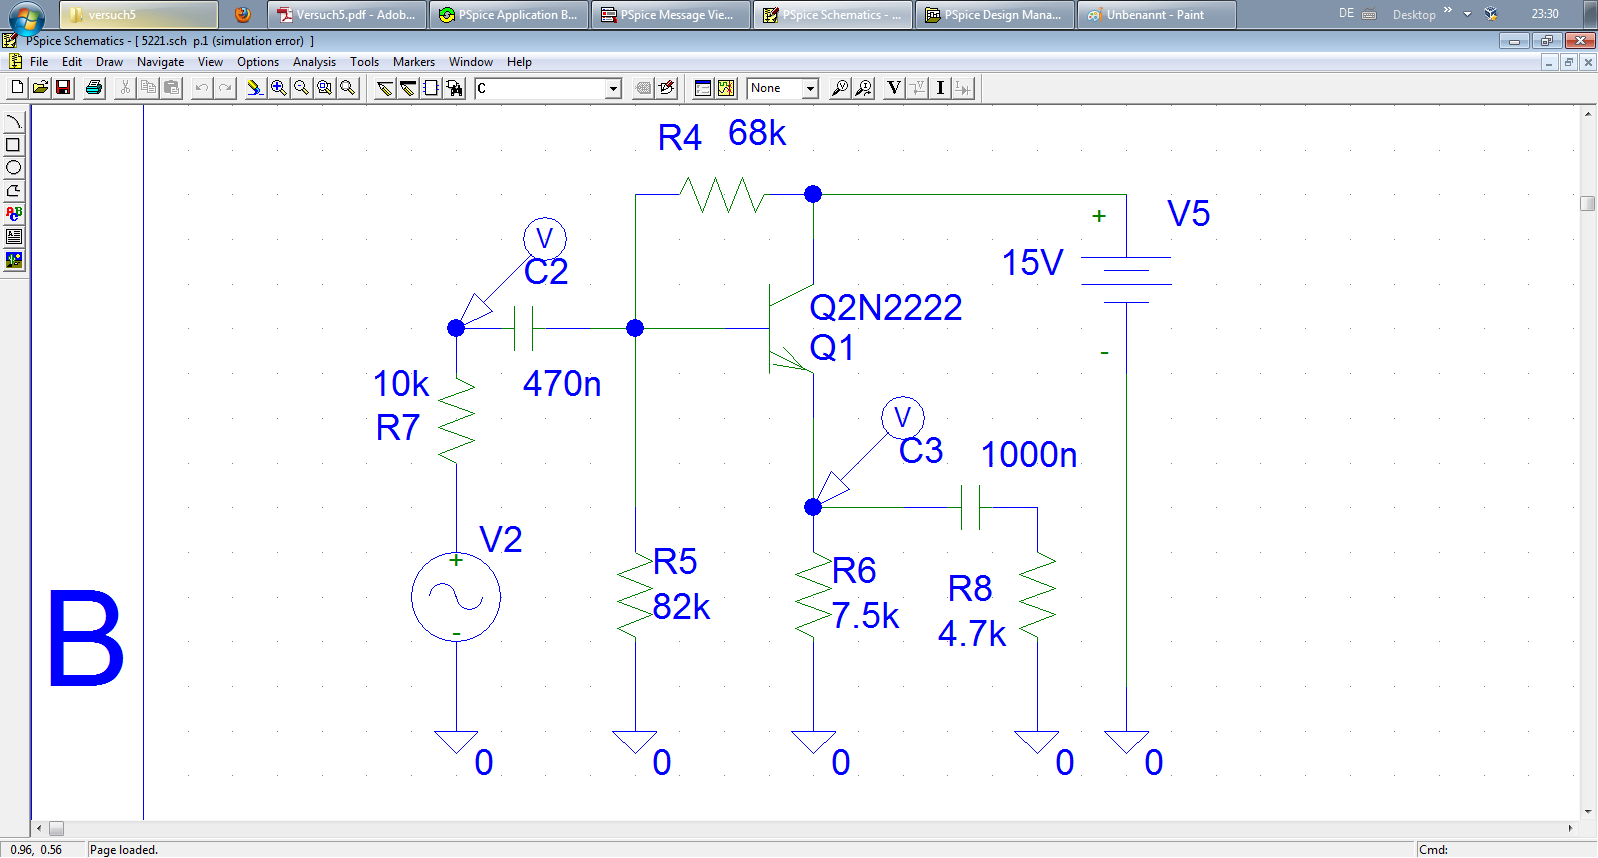
\includegraphics[width=\linewidth]{versuch5/spice/s5221.png}
	\caption{Schaltplan, wie im Skript vorgegeben}
\end{figure}
\begin{figure}[H]
	\centering
	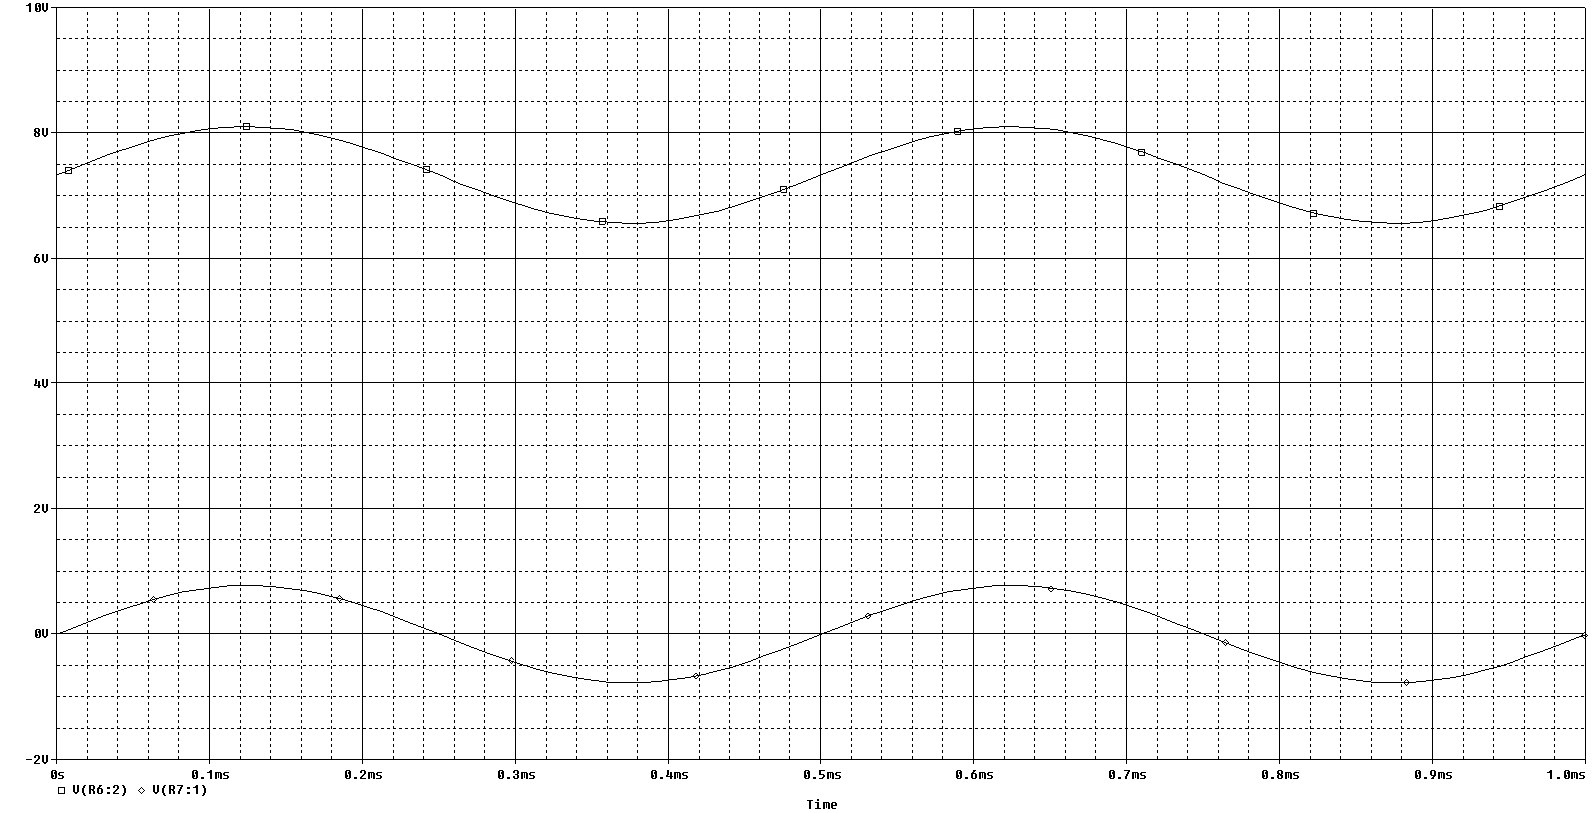
\includegraphics[width=\linewidth]{versuch5/spice/5221.png}
	\caption{Simulationsergebnis}
\end{figure}
Als Nächstes habe ich die Amplitude auf 10V erhöht. Dabei ergab sich folgender Spannungsverlauf:
\begin{figure}[H]
	\centering
	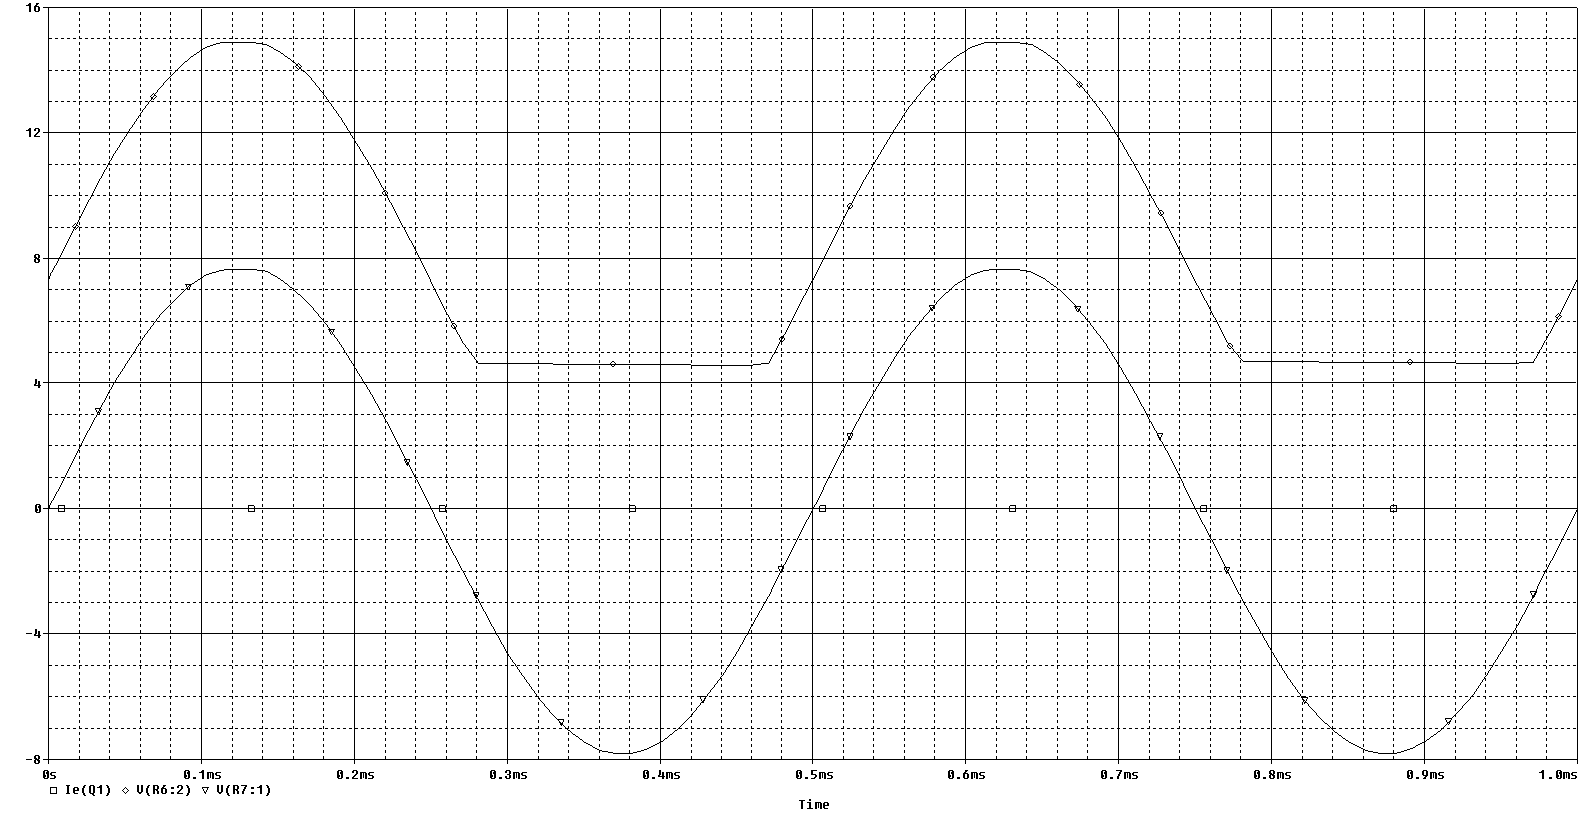
\includegraphics[width=\linewidth]{versuch5/spice/5222.png}
	\caption{Simulationsergebnis}
\end{figure}
\begin{figure}[H]
	\centering
	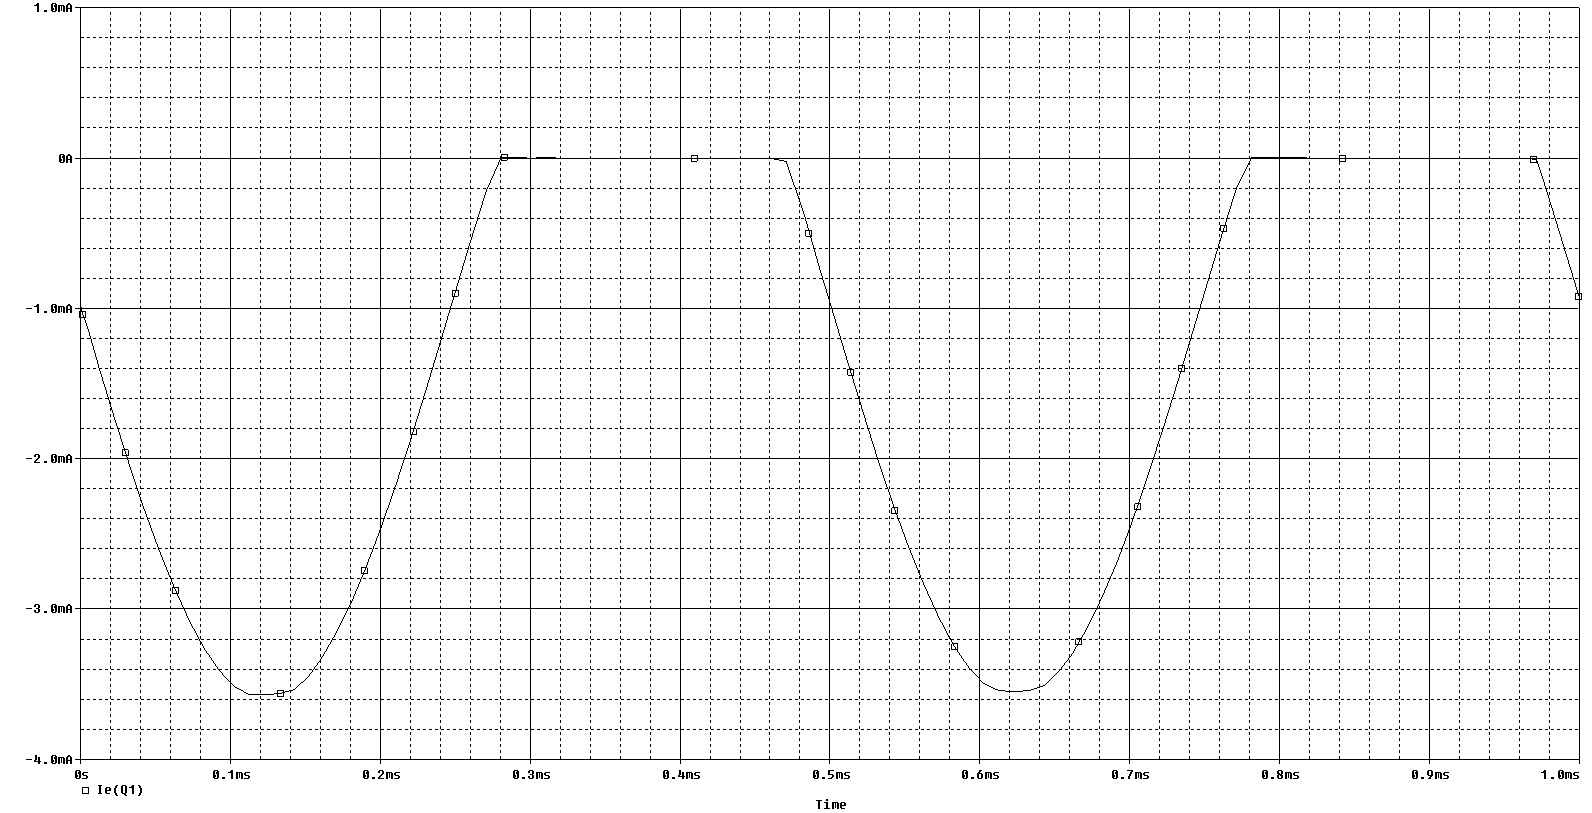
\includegraphics[width=\linewidth]{versuch5/spice/5222I.png}
	\caption{Simulationsergebnis: Nur Strom}
\end{figure}
Es zeigen sich deutlich die Clipping-Effekte bei einer Ausgangsspannung unterhalb 4.65V.\\
Dieser Effekt rührt daher, dass der Kondensator C3 das Spannungsnieveau hält. bei den 4.65V trifft die (steigende) Ladekurve des Kondensators auf die (fallende) Spannungskurve des variablen Widerstandsteilers aus Q1 und R6, daher erscheint ein deutlich sichtbarer Knick im Verlauf der Ausgangsspannung. Um die Spannung auch auf der negativen Halbwelle tiefer einstellen zu können müsste R6 kleiner gewählt sein (mit allen Folgen), oder man verwendet gleich auch einen Transistor, dann lässt sich auch eine kapazitive Last mit weniger Verzerrungen ansteuern.

Bei niedrigen Frequenzen dominiert die Hochpasscharakteristik des Filters aus R7, C2 und R5. Das Eingangssignal wird also vom Filter gedämpft, daher wird der Transistor nicht voll angesteuert und somit ist die Verstärkung insgesammt eher schwach, obwohl der Transistor an sich mit den niedrigen Frequenzen kein Problem hätte.\\
Die Amplitude des Eingangssignals steigt bei niedrigen Frequenzen an, weil der Kondensator dort hochohmig(-er) ist. Somit wird die Reale Spannungsquelle aus V2 und R7 schwächer belastet und kommt somit iher Leerlaufspannung näher.
\subsubsection*{Messung}
Die aufgebaute Platine lieferte folgende Ausgangsspannung:
\begin{figure}[H]
	\centering
	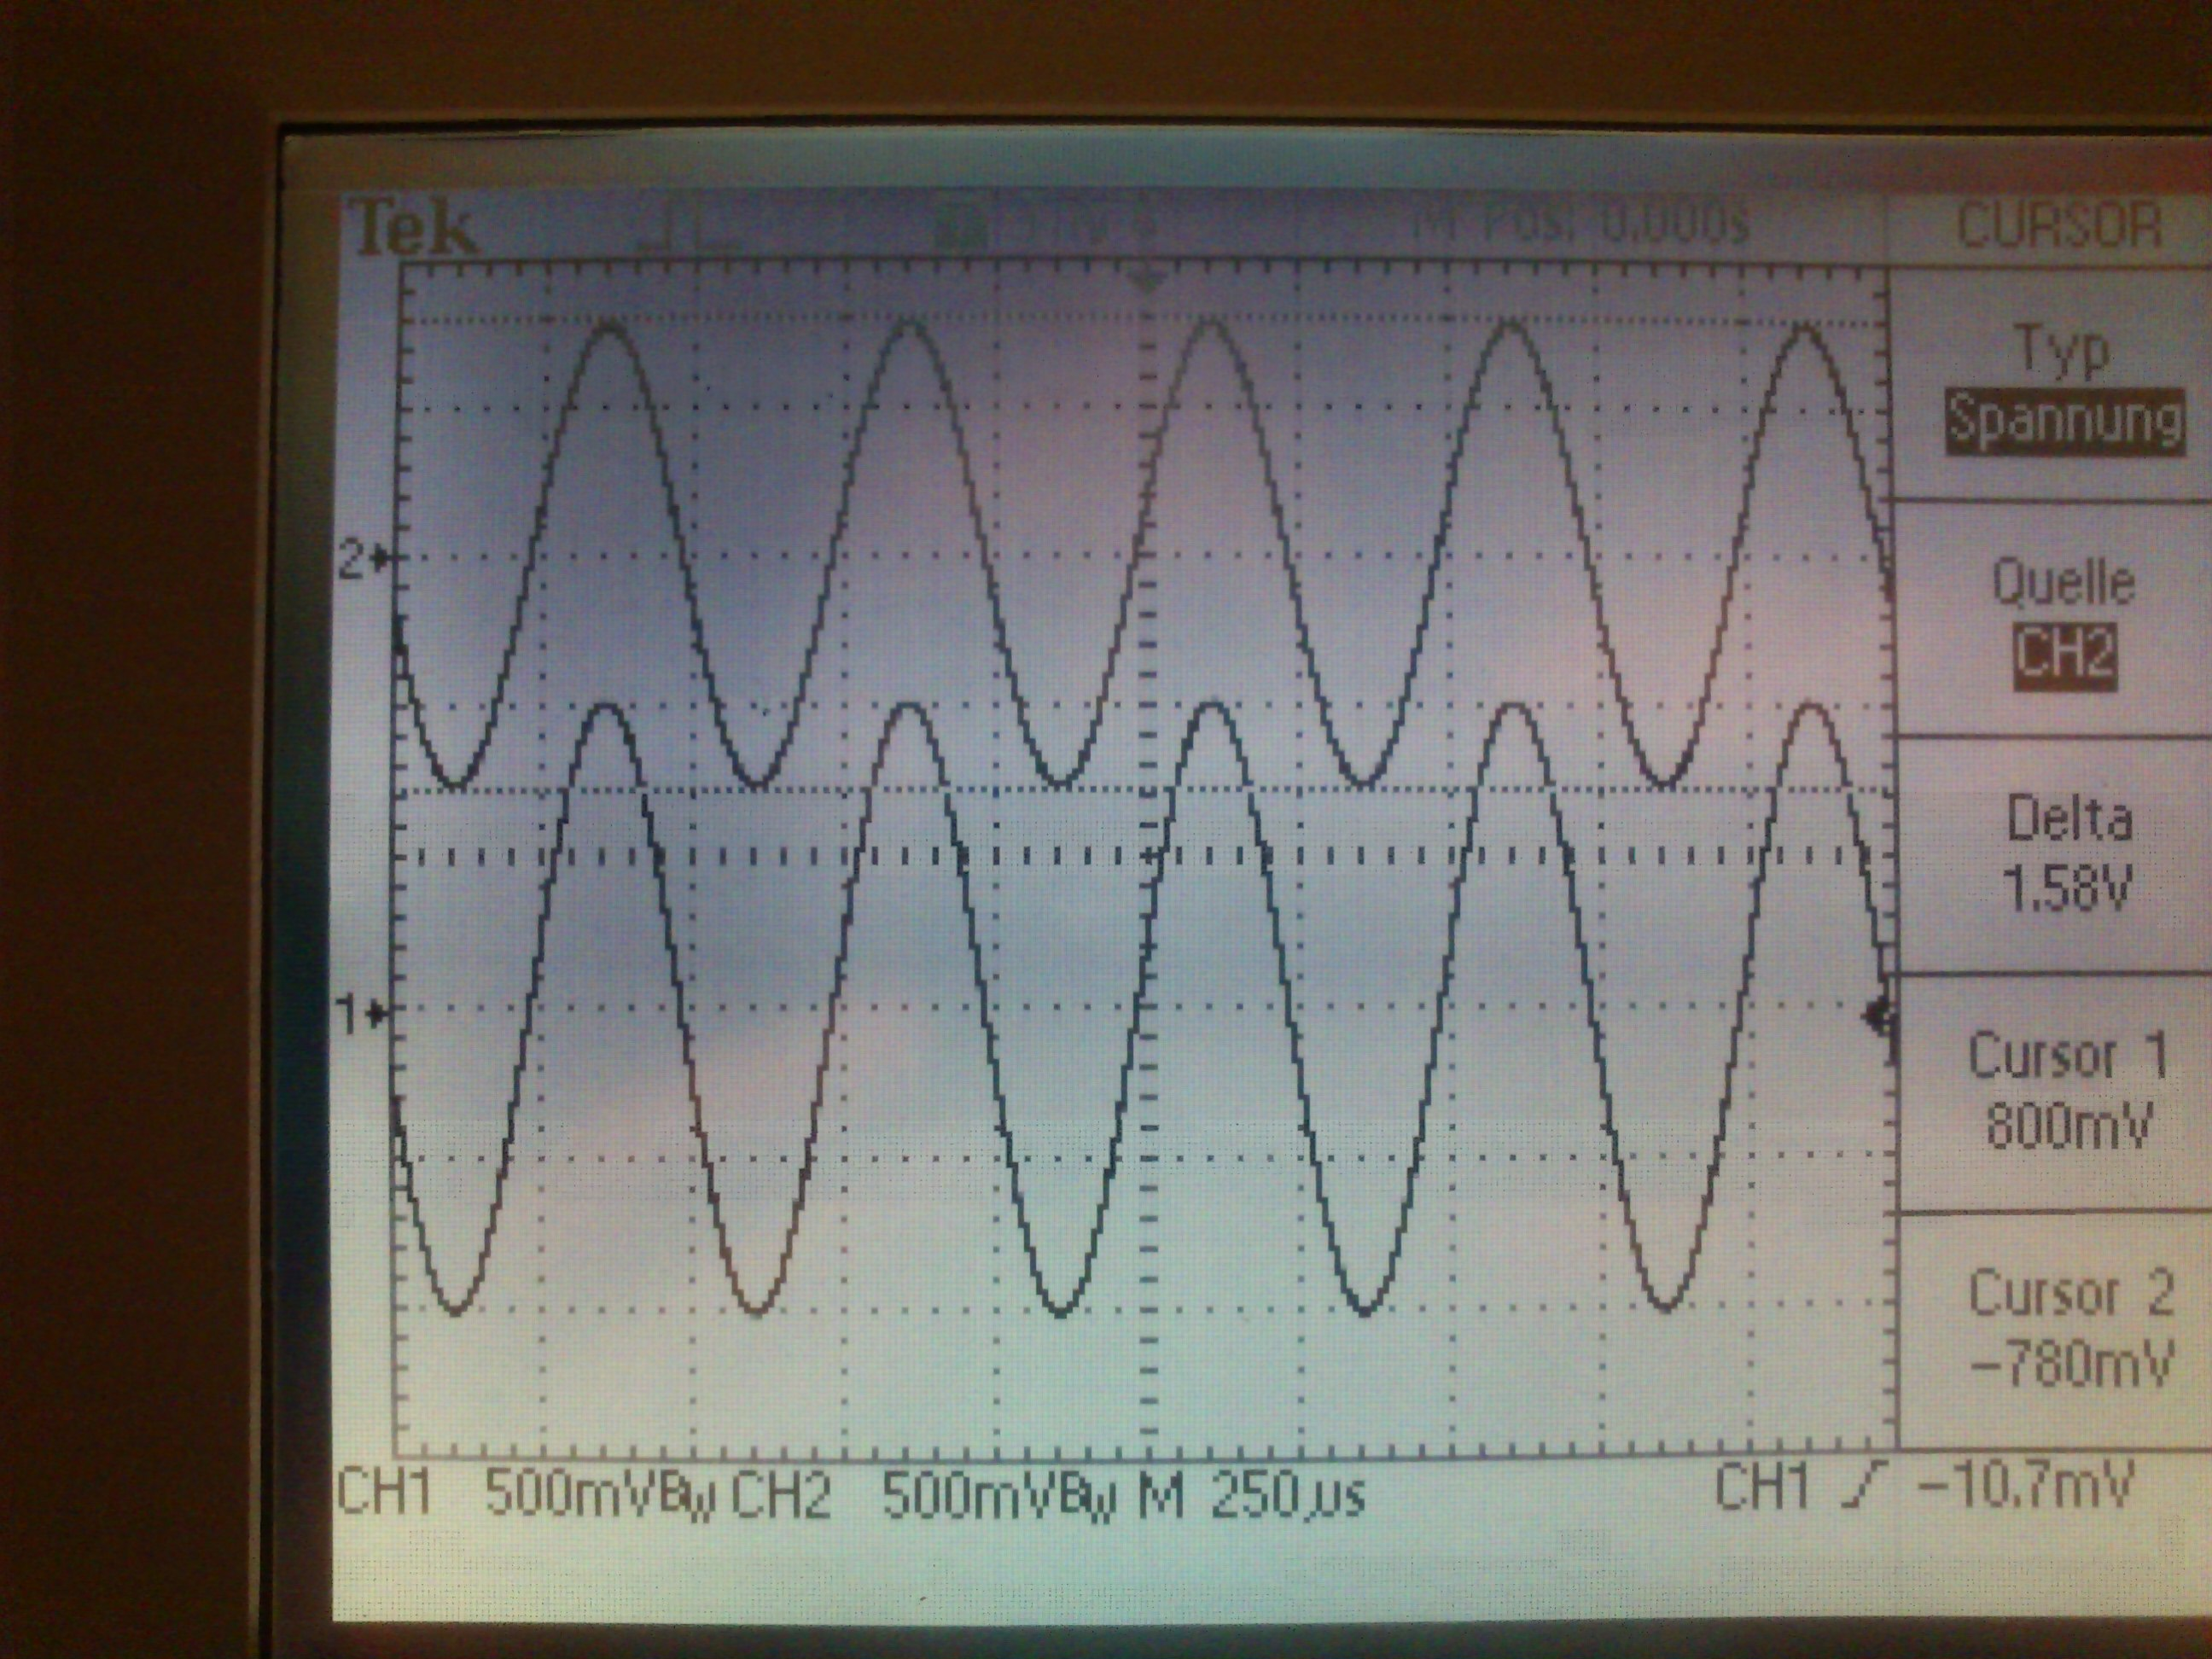
\includegraphics[width=\linewidth]{versuch5/oszi/DSC_0444.JPG}
	\caption{Ausgangsspannung bei 2kHz: 1.58V, Eingangsspannung: 1.02V}
\end{figure}
Die reale Schaltung liefert mehr Spannung als erwartet. Es ergibt sich somit ein Verstärkungsfaktor von $\frac{1.58}{1.02}=1.549\approx1.55$.


\subsection{Entwurf, Simulation und Aufbau eines Transistorverstärkers (Emitterschaltung)}
\subsubsection*{Simulation}
Die Bauteilwerte wurden wie folgt bestimmt:\\
\begin{tabular}{ll}
	Bauteil & Wert\\
	\hline
	C1 & 79.6nF, verwendet 220nF\\
	C2 & 9.3 \mikro F, verwendet 22 \µF\\
	R1 & 100k\Ohm\\
	R2 & 8.2k\Ohm, verwendet: 9.1k\Ohm\\
	R3 & 171.43\Ohm\\
	RC & 20k\Ohm\\
	RE & 2k\Ohm\\
\end{tabular}

\begin{figure}[H]
	\centering
	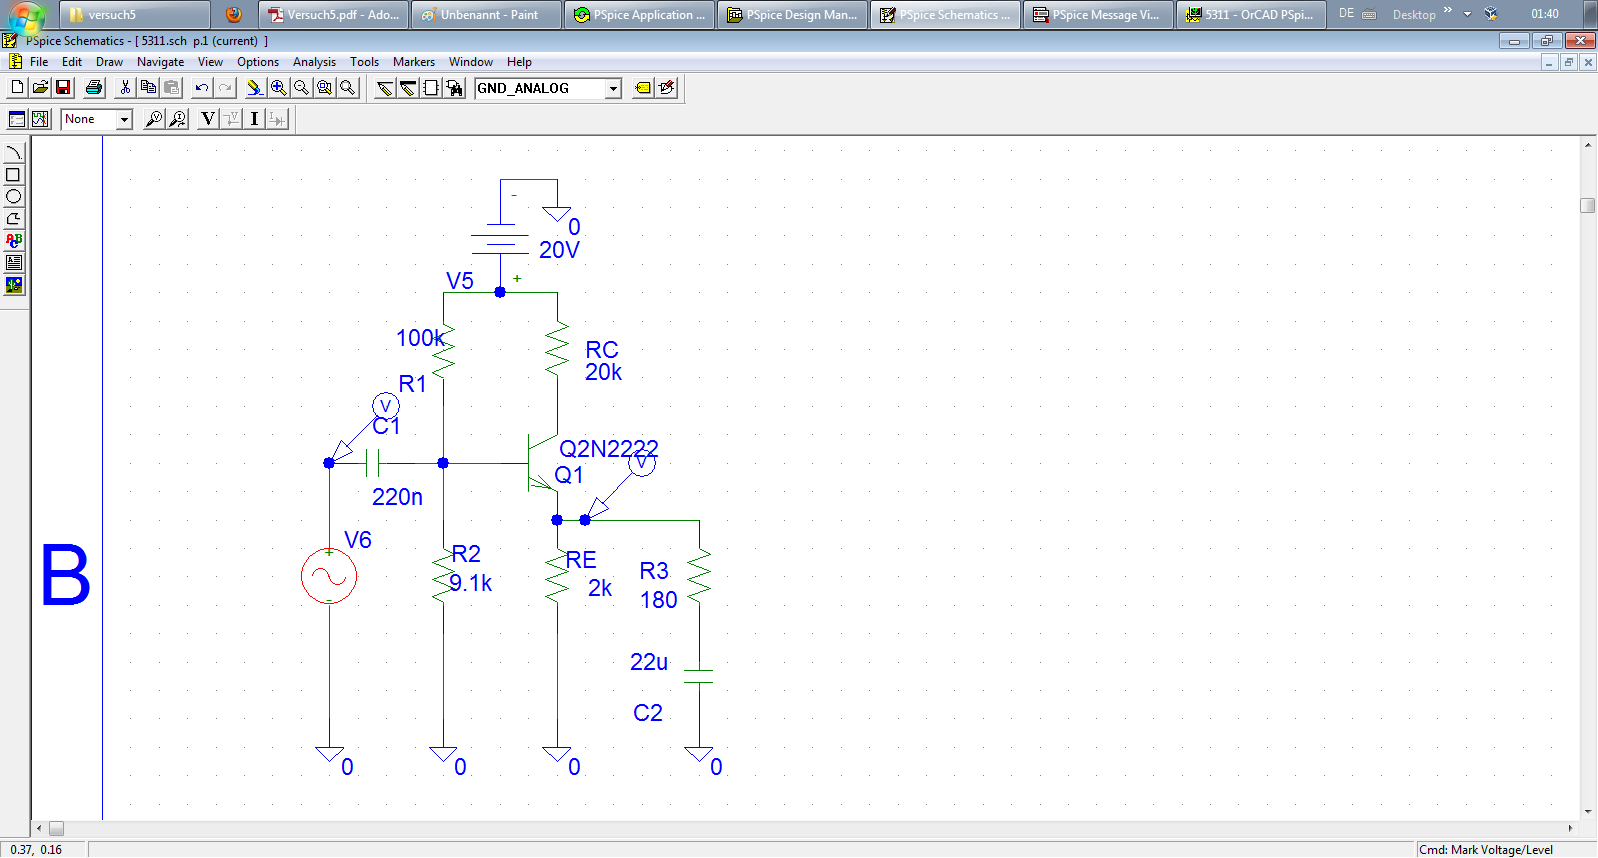
\includegraphics[width=\linewidth]{versuch5/spice/s5312.png}
	\caption{Schaltplan, wie im Skript vorgegeben}
\end{figure}
\begin{figure}[H]
	\centering
	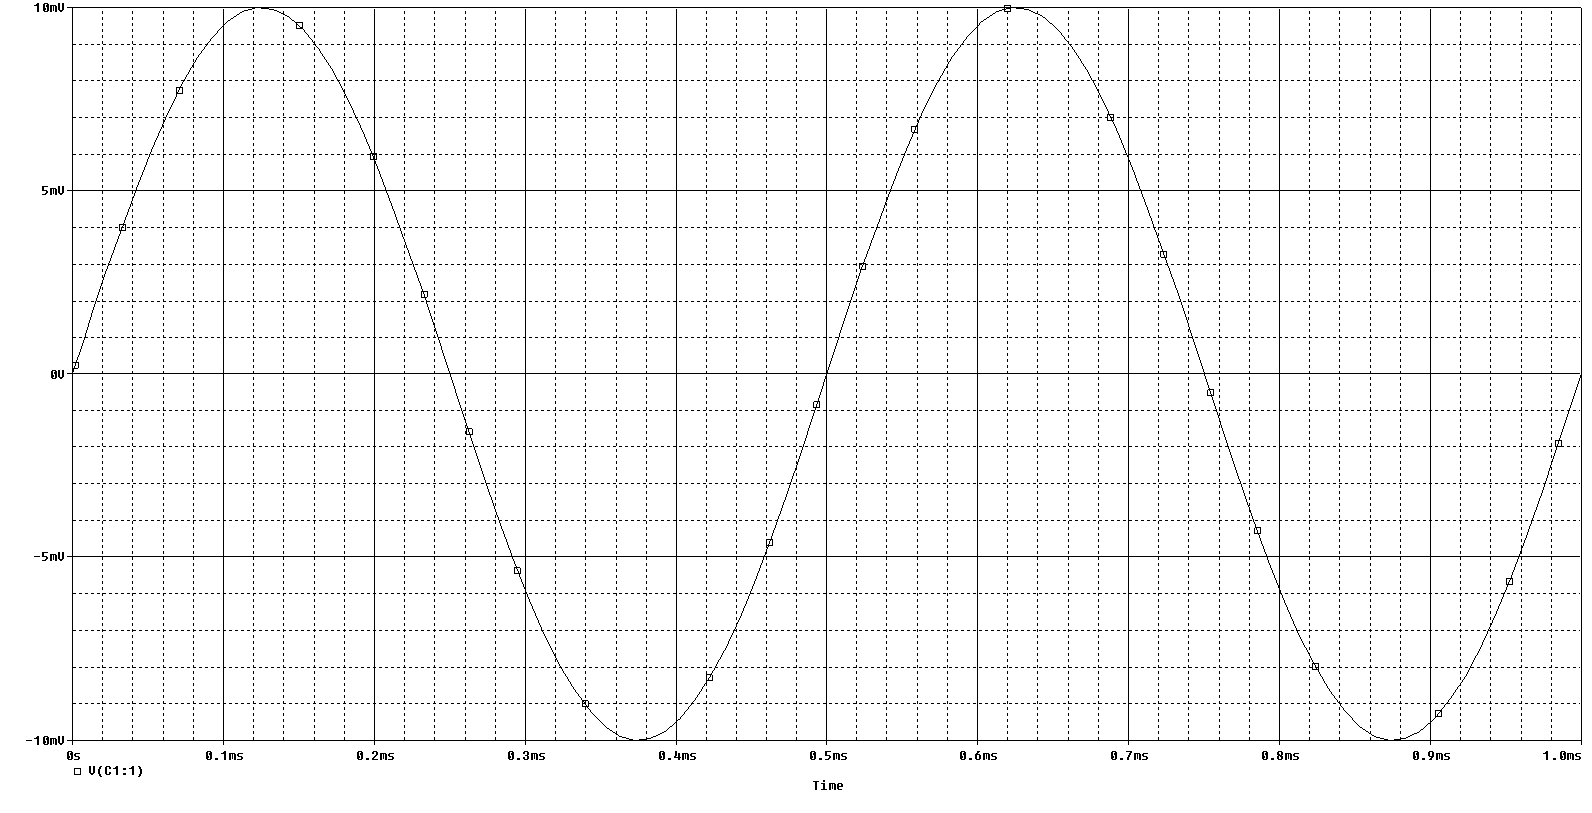
\includegraphics[width=\linewidth]{versuch5/spice/5311e.png}
	\caption{Simulationsergebnis: Eingangsspannung}
\end{figure}
\begin{figure}[H]
	\centering
	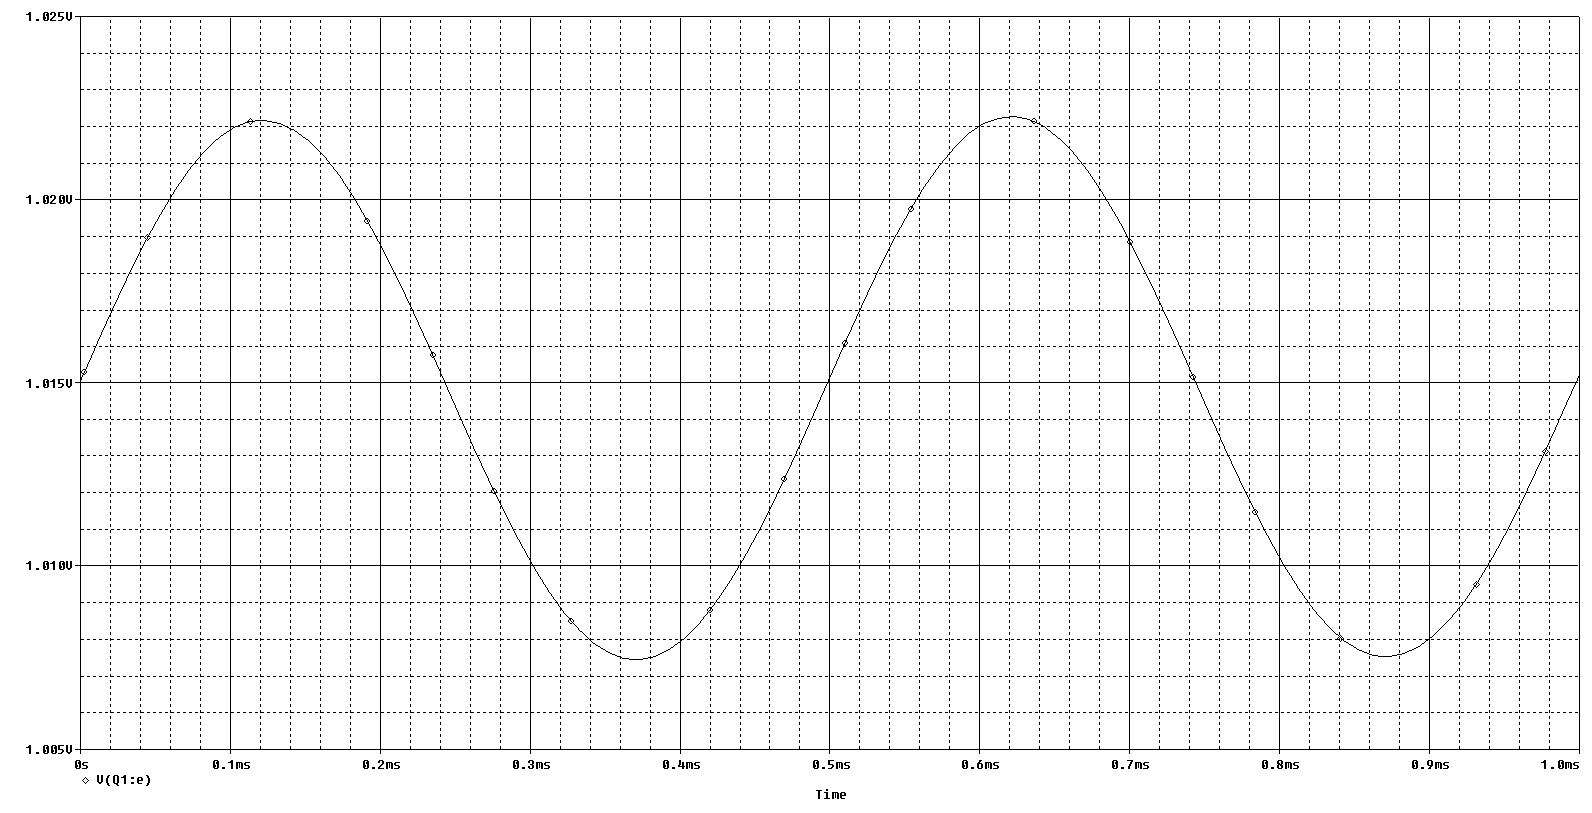
\includegraphics[width=\linewidth]{versuch5/spice/5311a.png}
	\caption{Simulationsergebnis: Ausgangsspannung}
\end{figure}
Die simulierte Verstärkung ist $\frac{1.22}{0.01}=122$.\\
Als nächstes habe ich die Amplitude der Signalquelle verzehnfacht:
\begin{figure}[H]
	\centering
	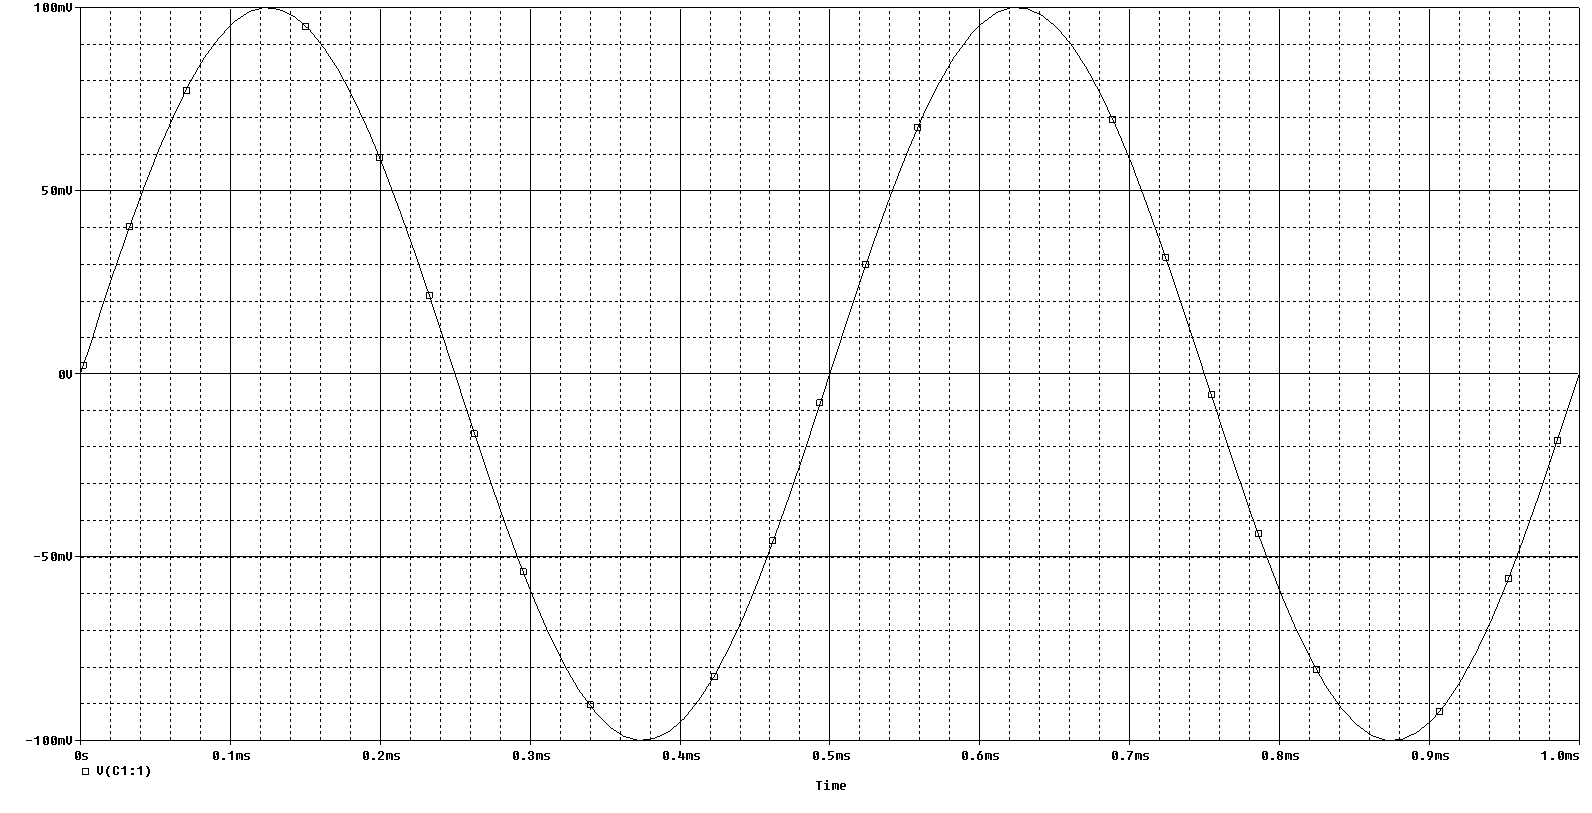
\includegraphics[width=\linewidth]{versuch5/spice/5312e.png}
	\caption{Simulationsergebnis: Eingangsspannung}
\end{figure}
\begin{figure}[H]
	\centering
	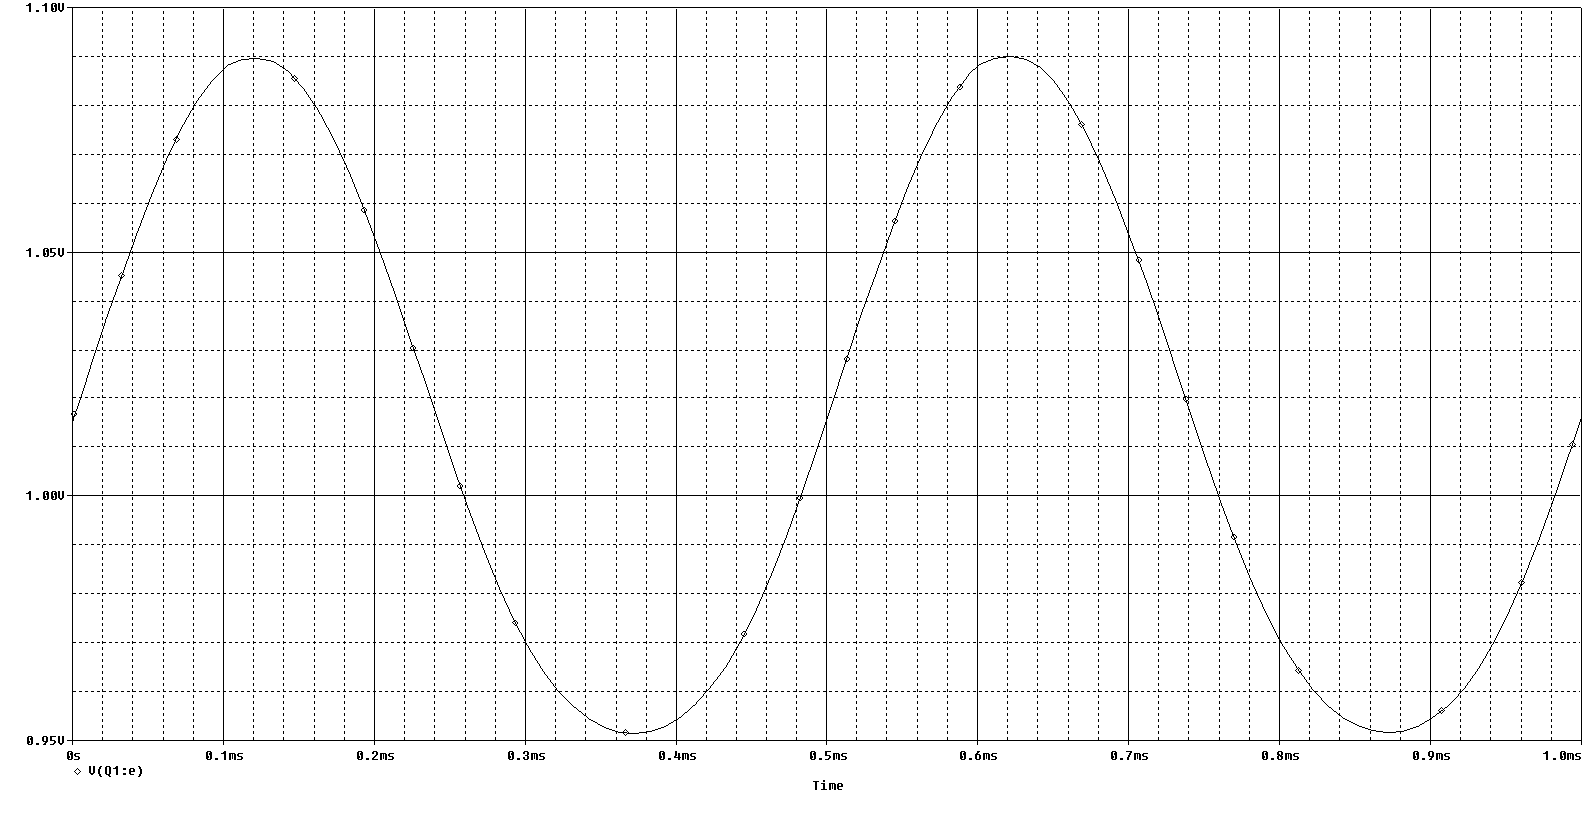
\includegraphics[width=\linewidth]{versuch5/spice/5312a.png}
	\caption{Simulationsergebnis: Ausgangsspannung}
\end{figure}
Man sieht deutlich, dass der Mittelwert des Ausgangssignals durch die Bezugspunktverschiebung des Transistors nach oben verschoben wurde. Die Verzerrungen wurden noch im Frequenzbereich untersucht:
\begin{figure}[H]
	\centering
	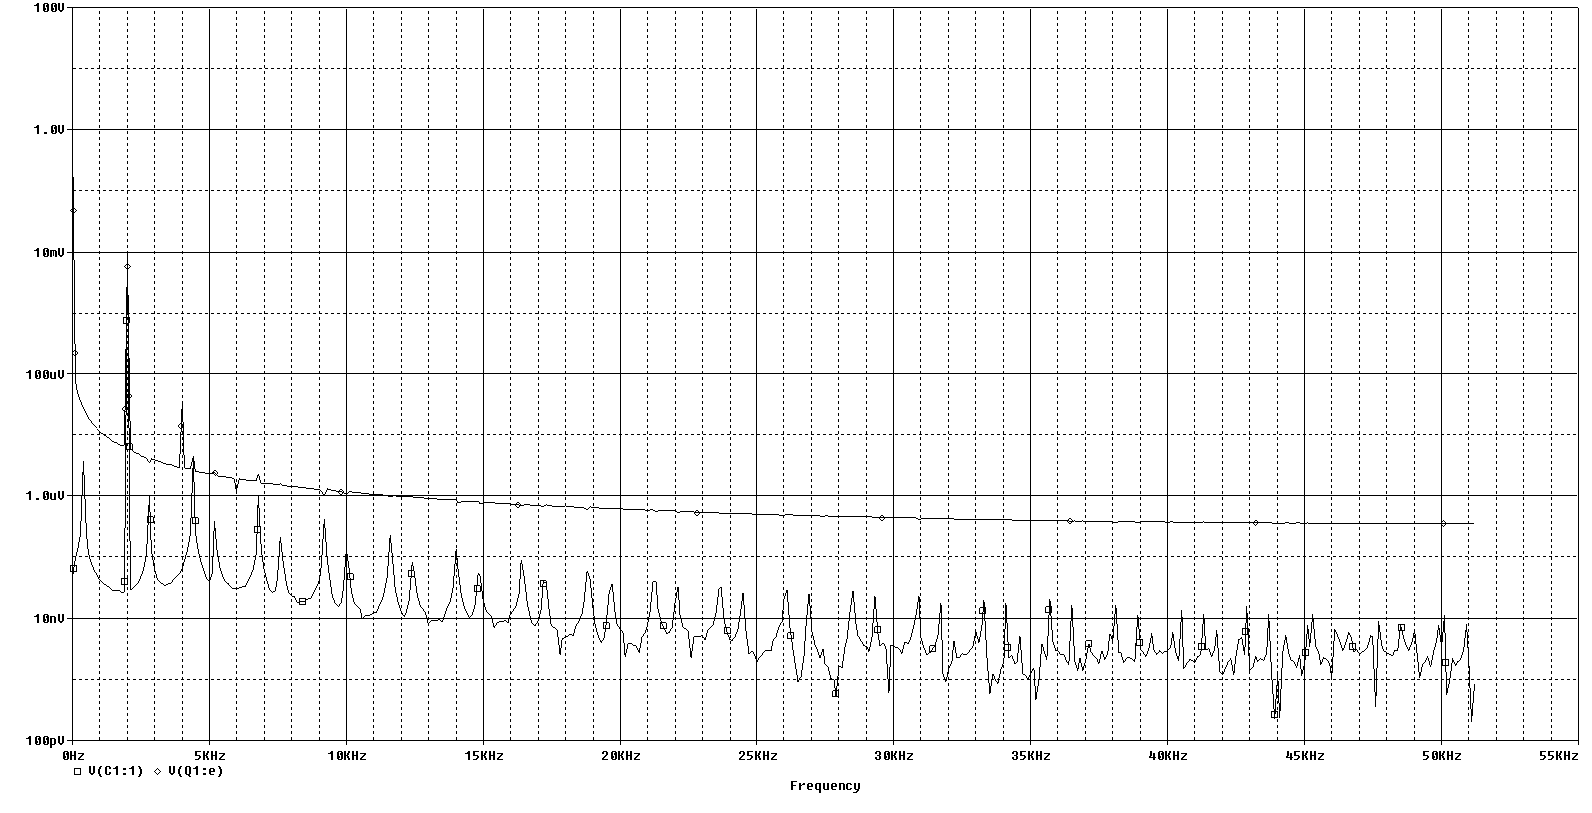
\includegraphics[width=\linewidth]{versuch5/spice/5313f1.png}
	\caption{Simulationsergebnis bei 10mV Eingangsspannung}
\end{figure}
\begin{figure}[H]
	\centering
	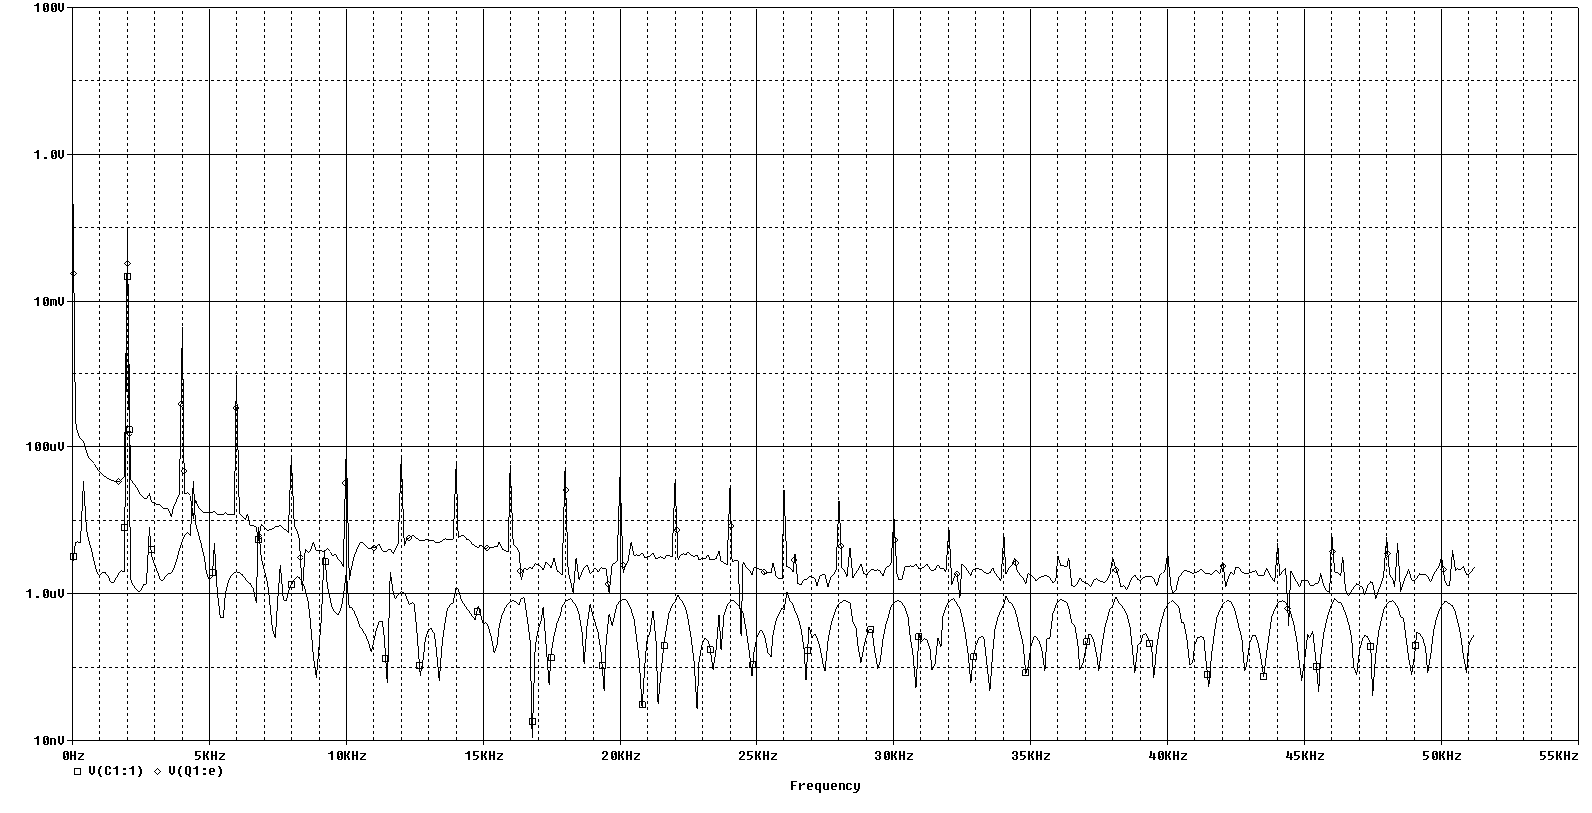
\includegraphics[width=\linewidth]{versuch5/spice/5313f2.png}
	\caption{Simulationsergebnis bei 100mV Eingangsspannung}
\end{figure}
Die Spitzenwerte der Oberwellen sind: 70mV, 45mV, 510\µ V, 100\µ V, 100\µ V. Daraus ergibt sich der Klirrfaktor wie folgt:
\[ \sqrt{\frac{\sum_{k=2}^5U_k^2}{\sum_{k=1}^5U_k^2}}=0.54 \]
Dann führte ich noch einen AC-Sweep aus:
\begin{figure}[H]
	\centering
	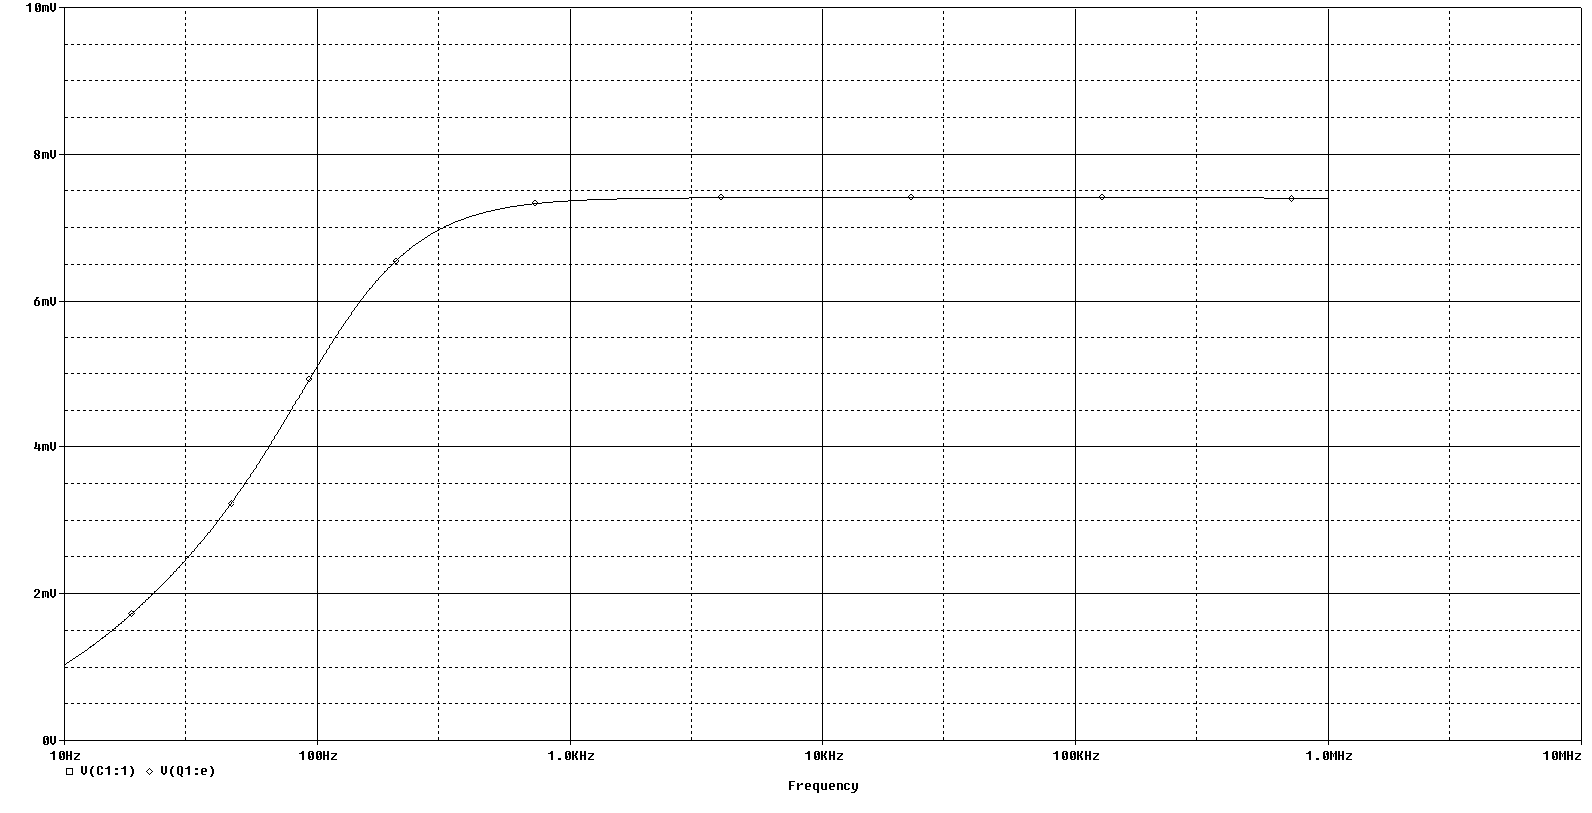
\includegraphics[width=\linewidth]{versuch5/spice/5314.png}
	\caption{Simulationsergebnis Ausgangsspannung im Abhängigkeit der Frequenz}
\end{figure}


\subsubsection*{Messung}
\begin{figure}[H]
	\centering
	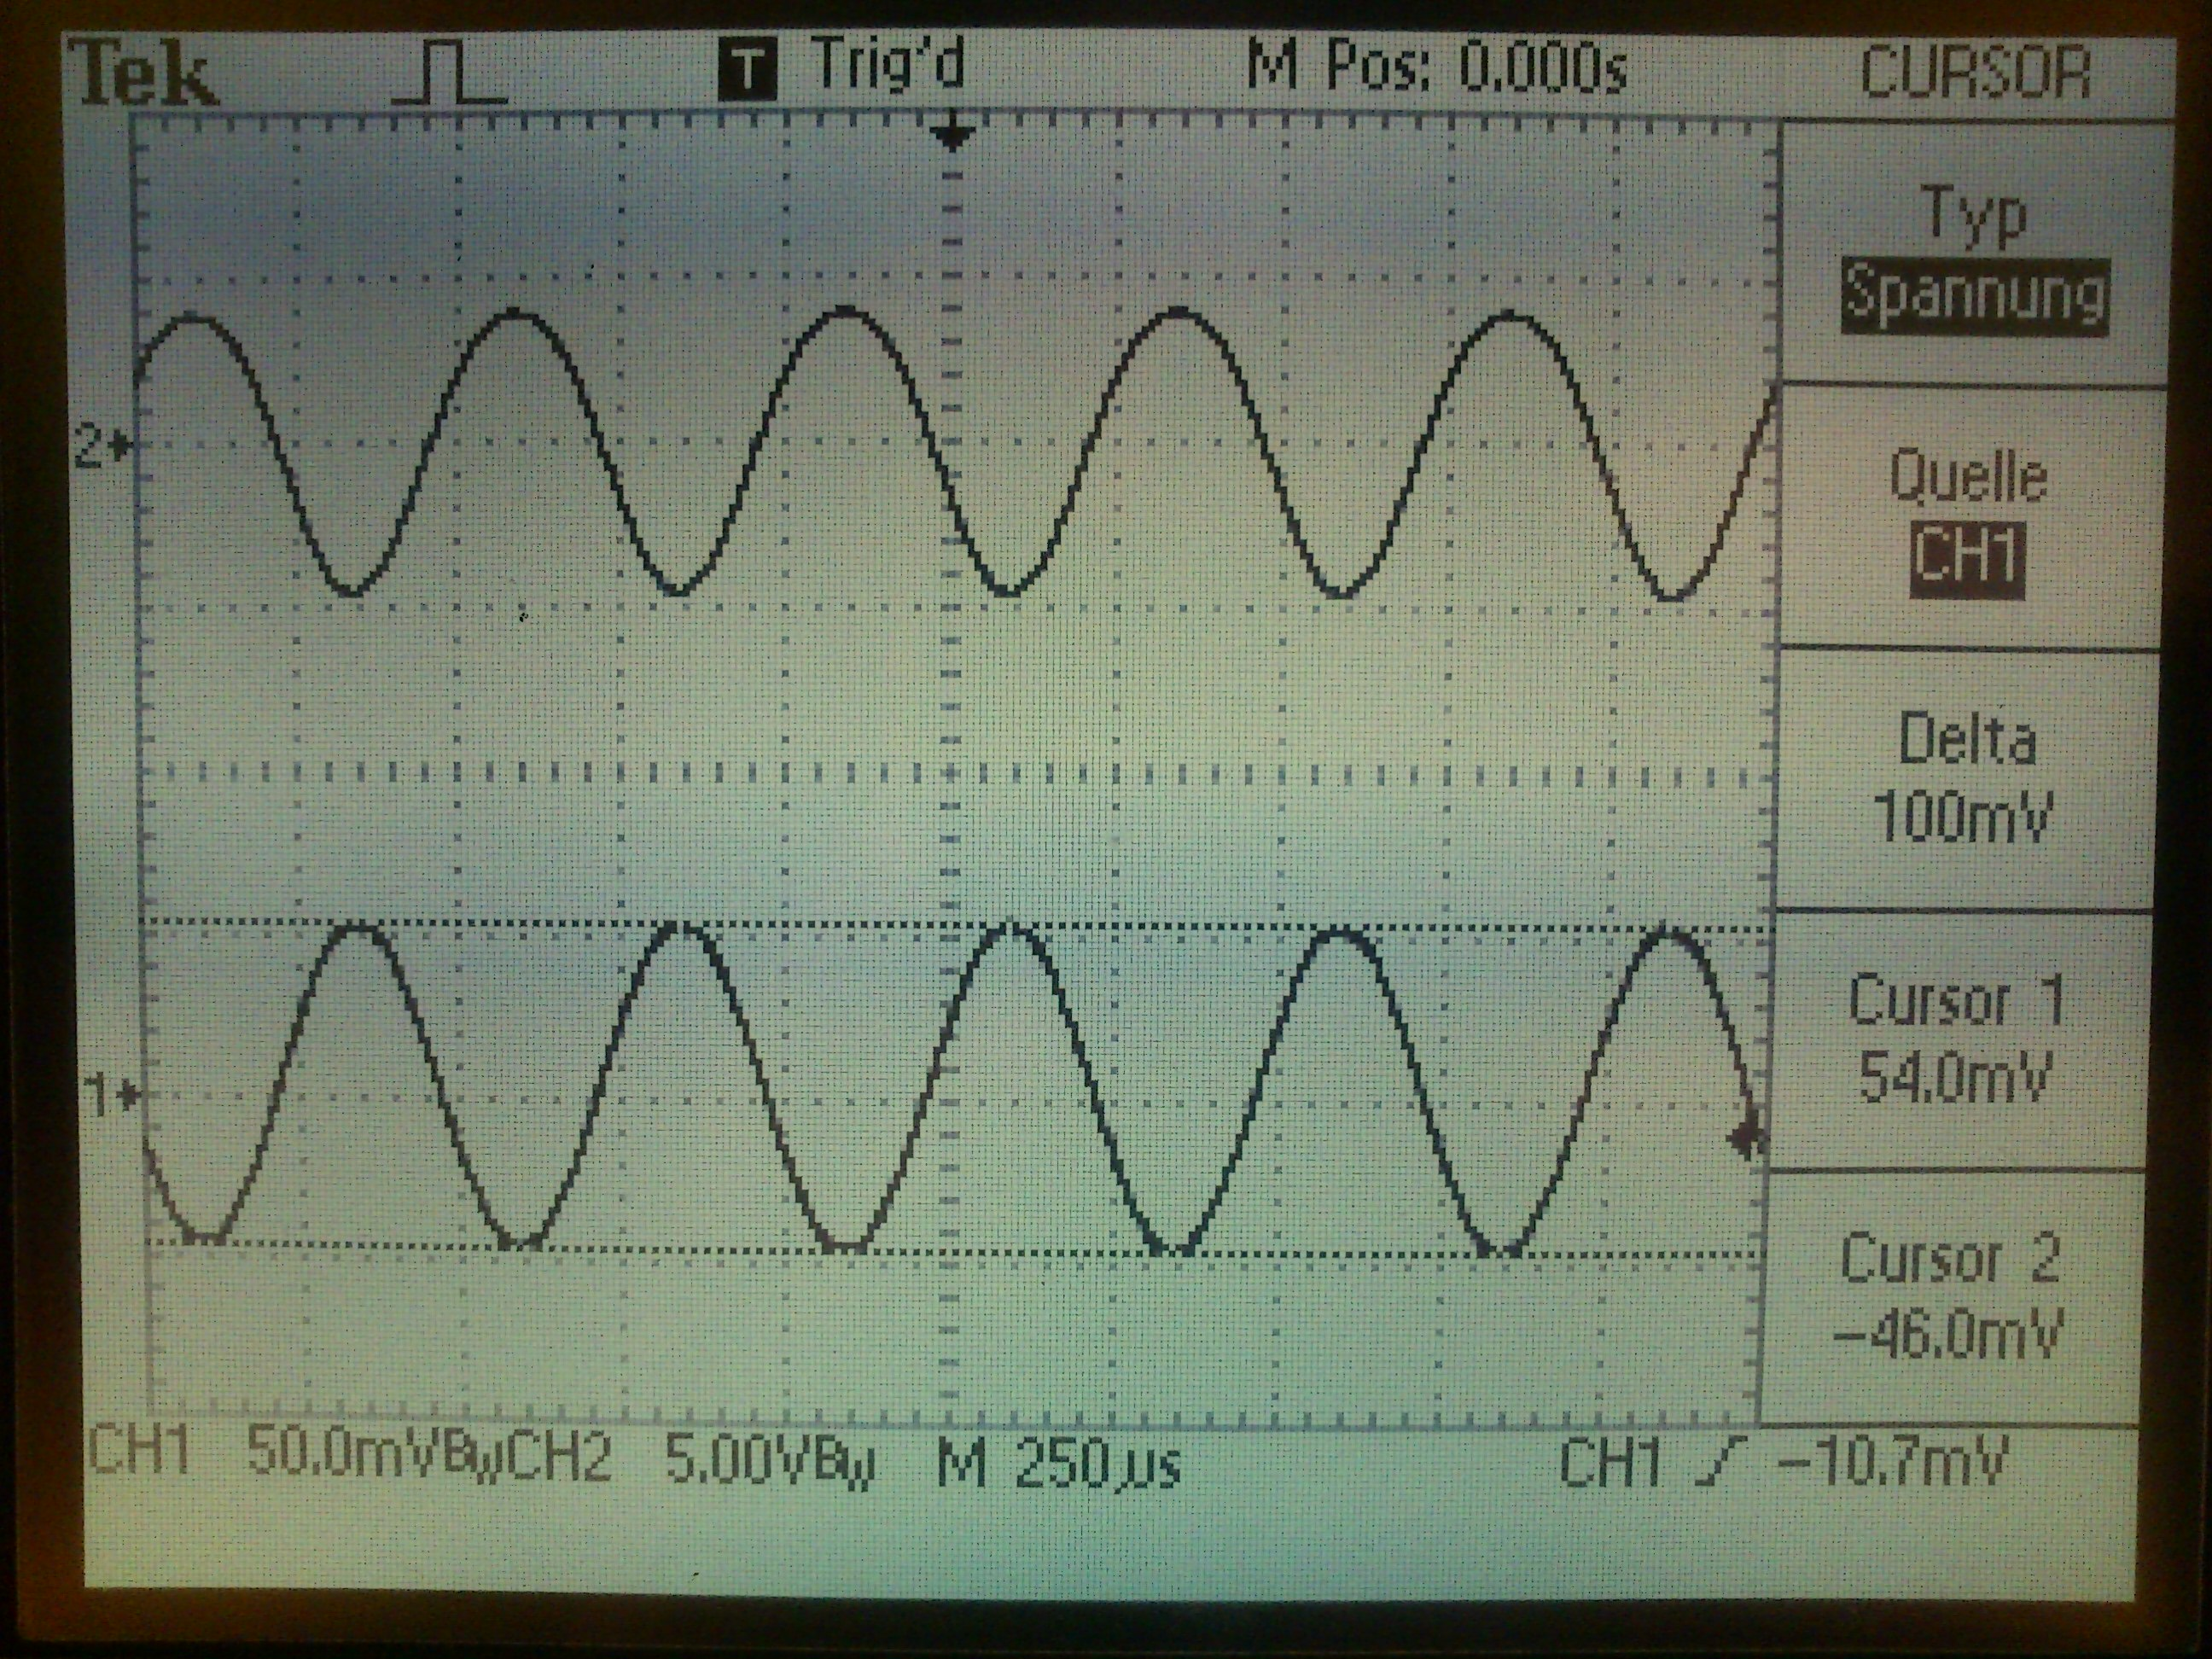
\includegraphics[width=\linewidth]{versuch5/oszi/DSC_0451.JPG}
	\caption{Bestimmung der Eingangsspannung zu 100mV}
\end{figure}
\begin{figure}[H]
	\centering
	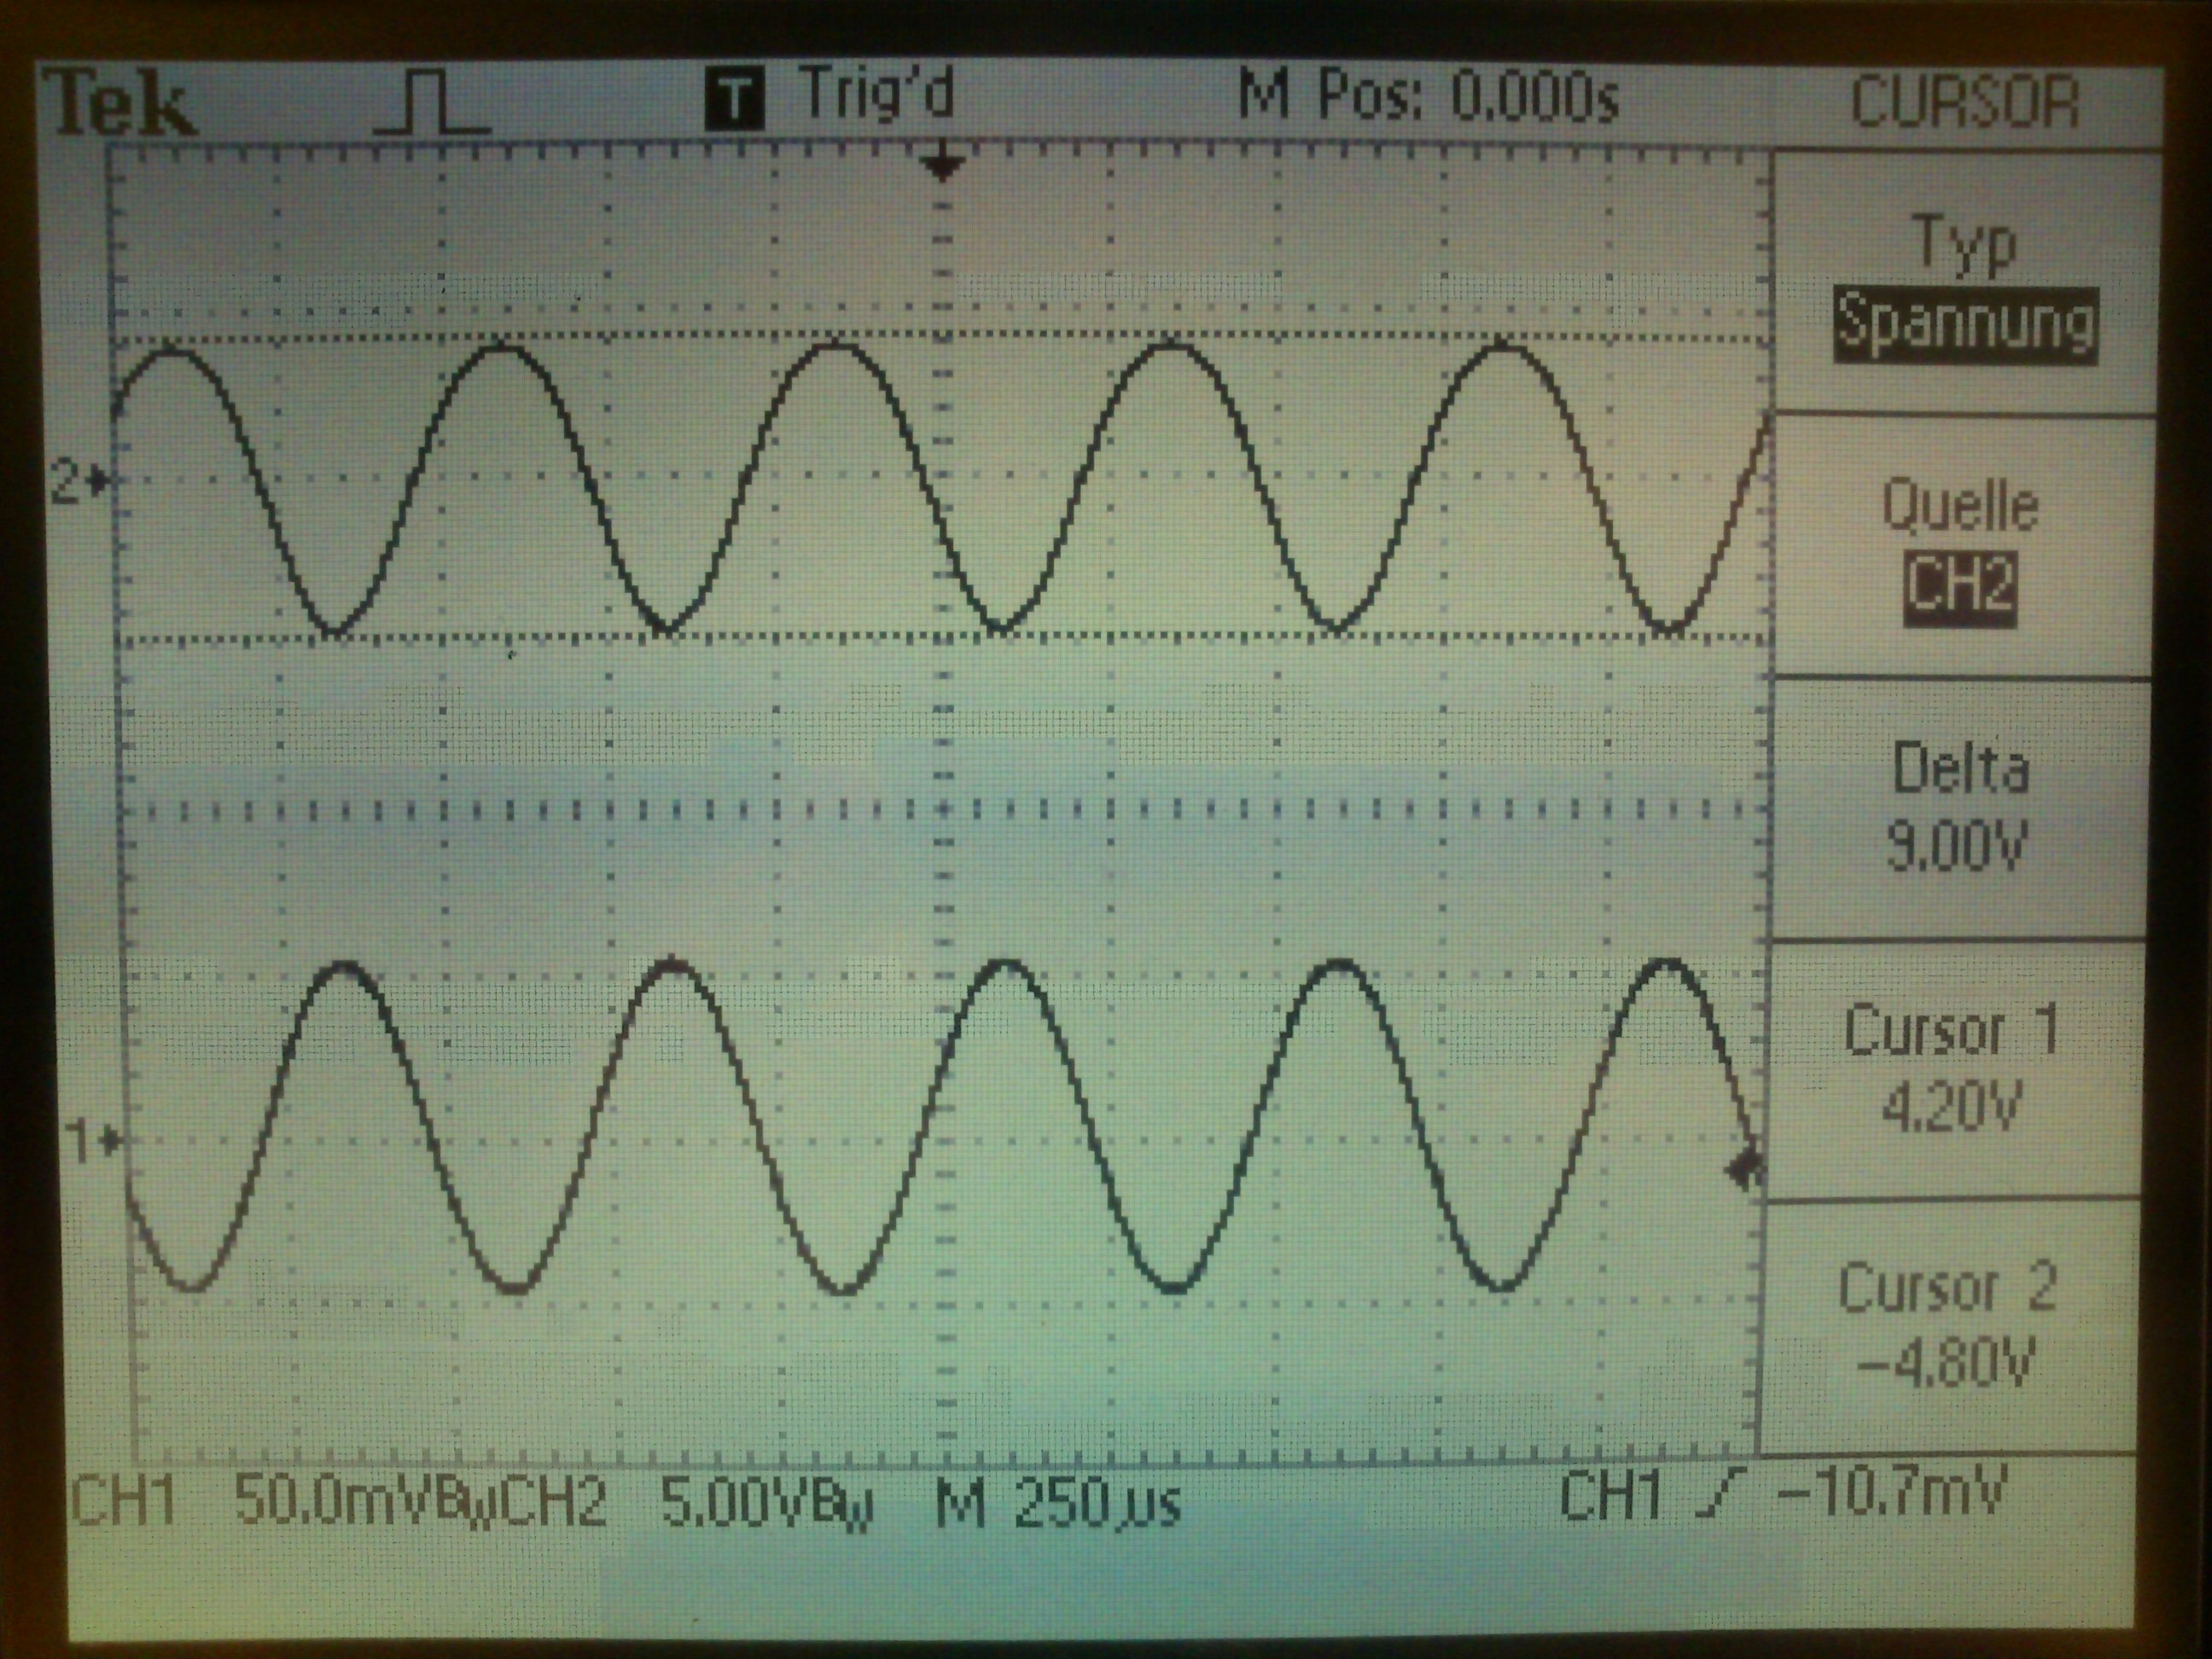
\includegraphics[width=\linewidth]{versuch5/oszi/DSC_0453.JPG}
	\caption{Bestimmung der Ausgangsspannung zu 9V}
\end{figure}
Daraus ergibt sich die Verstärkung zu $\frac{9V}{100mV}=90$ und bleibt damit weit hinter der Erwartung zurück. Die Grenzfrequenz des Verstärkers wurde zu 370kHz bestimmt.
\begin{figure}[H]
	\centering
	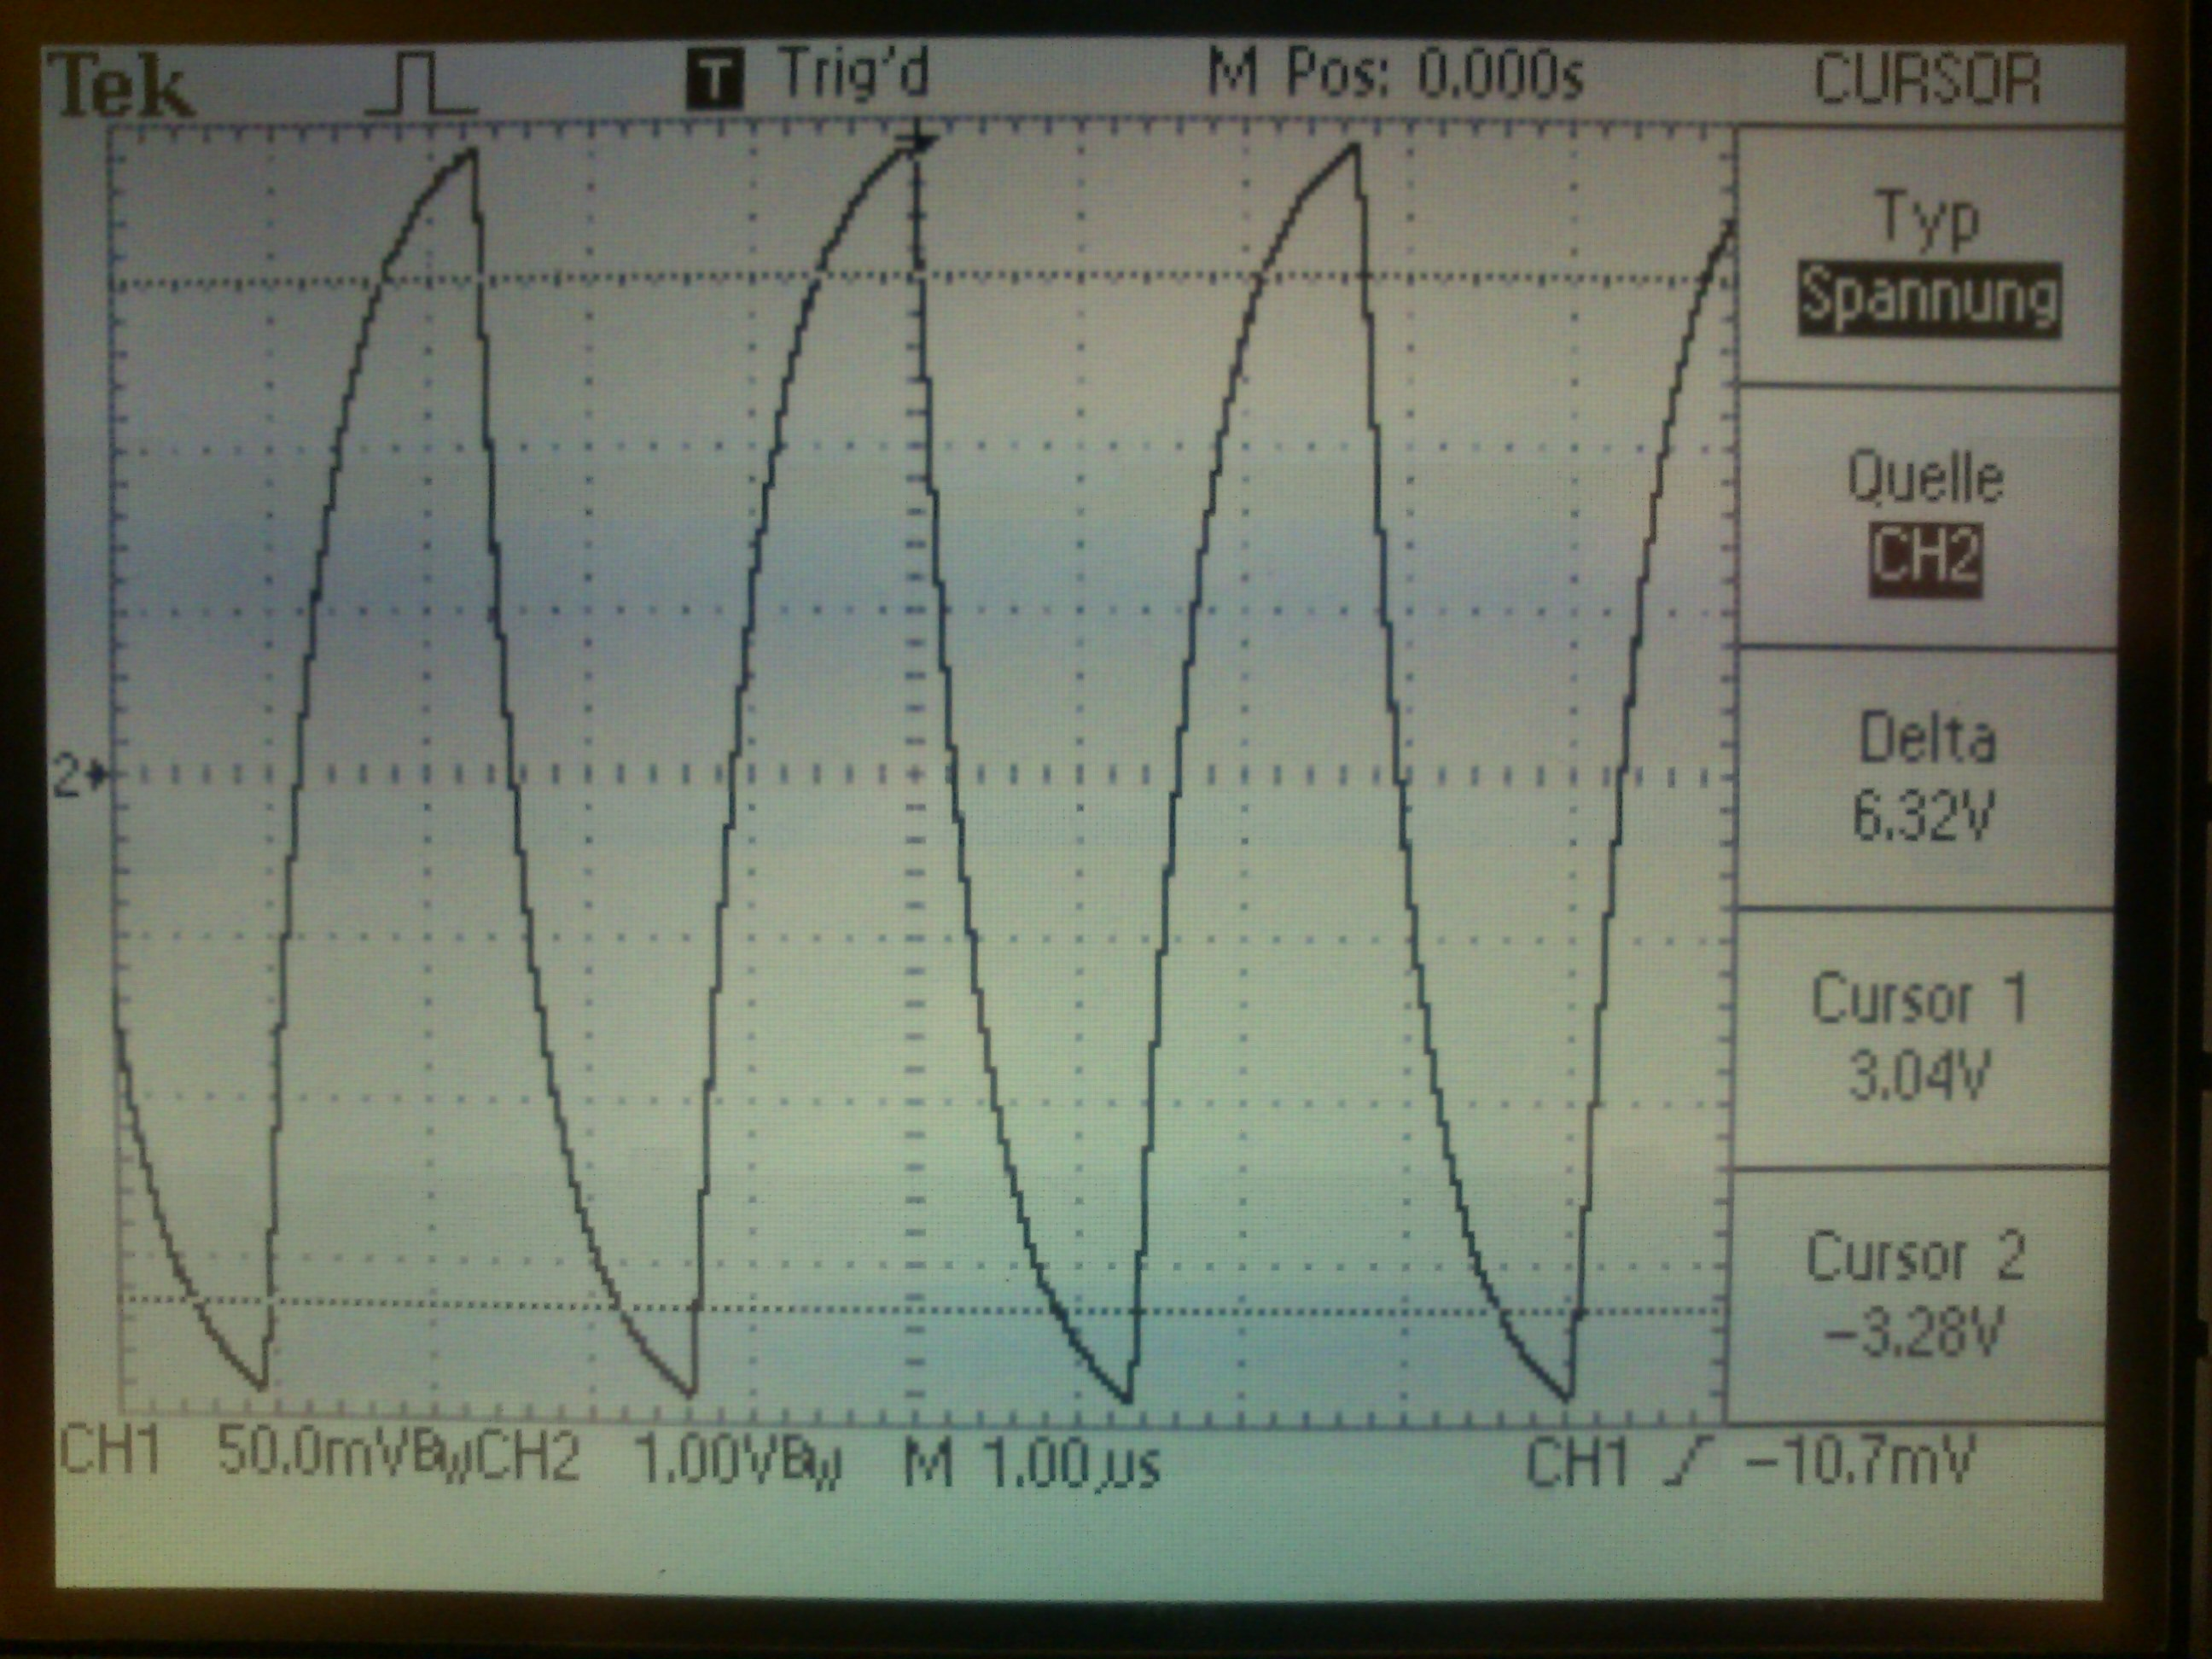
\includegraphics[width=\linewidth]{versuch5/oszi/DSC_0458.JPG}
	\caption{Signalform bei Rechteckspannung}
\end{figure}
Die Form kommt von der Hochpasscharakteristik des Eingangsfilters her. Die steilen Signalflanken können es quasi ungedämpft passieren, wärend die normalen Signale abgeschwächt werden.

Als nächstes wurde der Verstärker mit dem Digitalmultimeter verbunden und mit Kältespray behandelt. Die Spannungsverstärkung stieg dadurch an. Man sieht den Effekt nur 10 fach verstärkt, weil die Beschaltung den Transistor 'zähmt'. Durch die gesteigerte Amplitude verschiebt sich der Bezugspunkt stärker während jeder Schwingung und dämpft somit das Signal.

\subsection{Transistor als Schalter}
\begin{figure}[H]
	\centering
	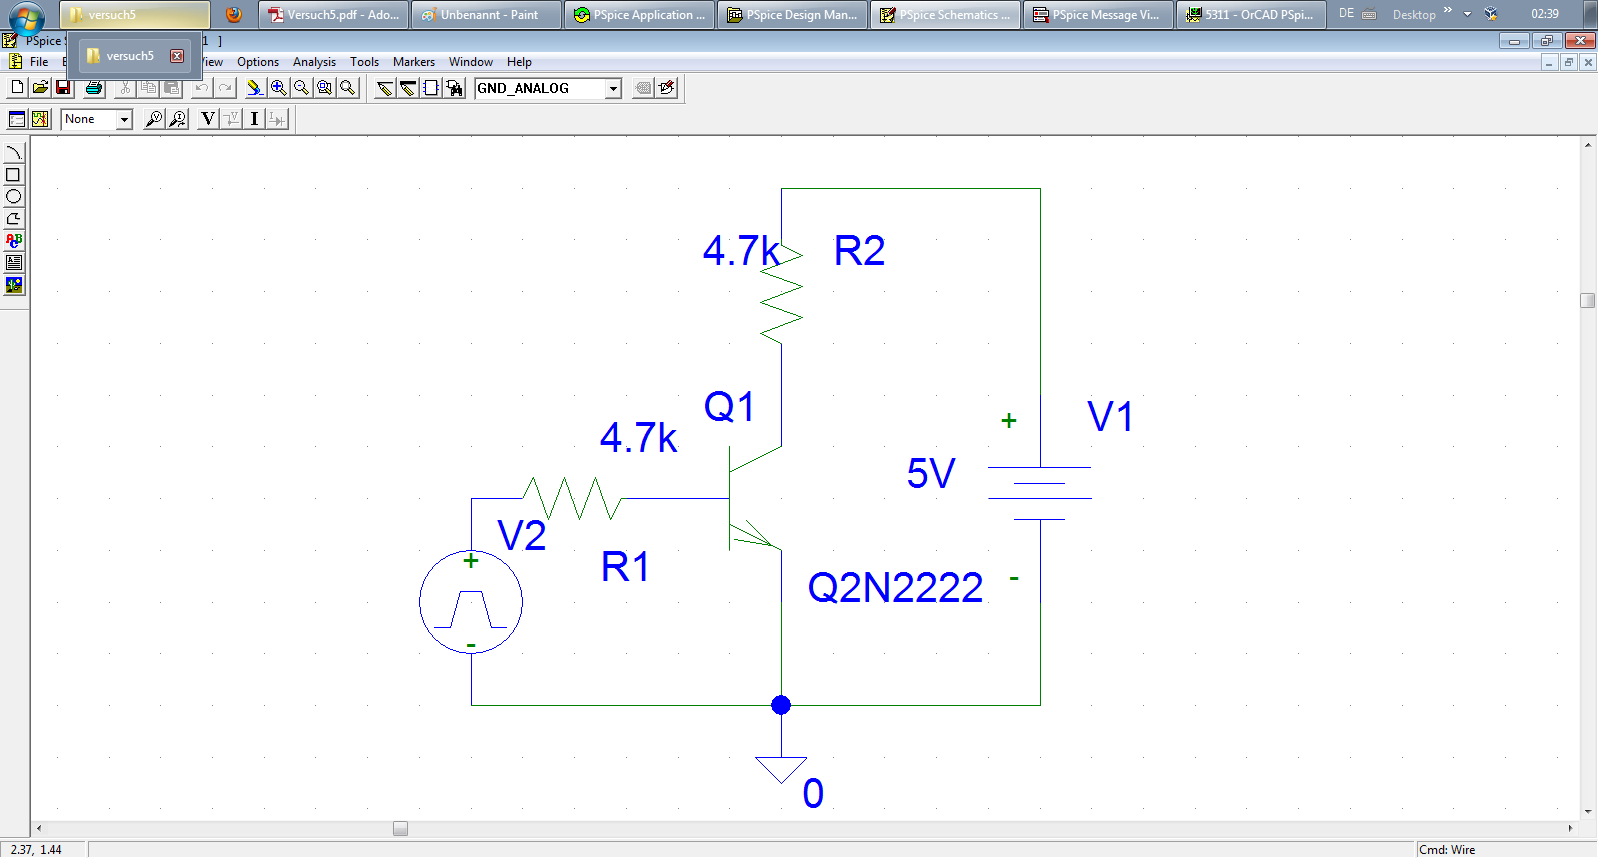
\includegraphics[width=\linewidth]{versuch5/spice/s5411.png}
	\caption{Schaltplan, wie im Skript vorgegeben}
\end{figure}
\begin{figure}[H]
	\centering
	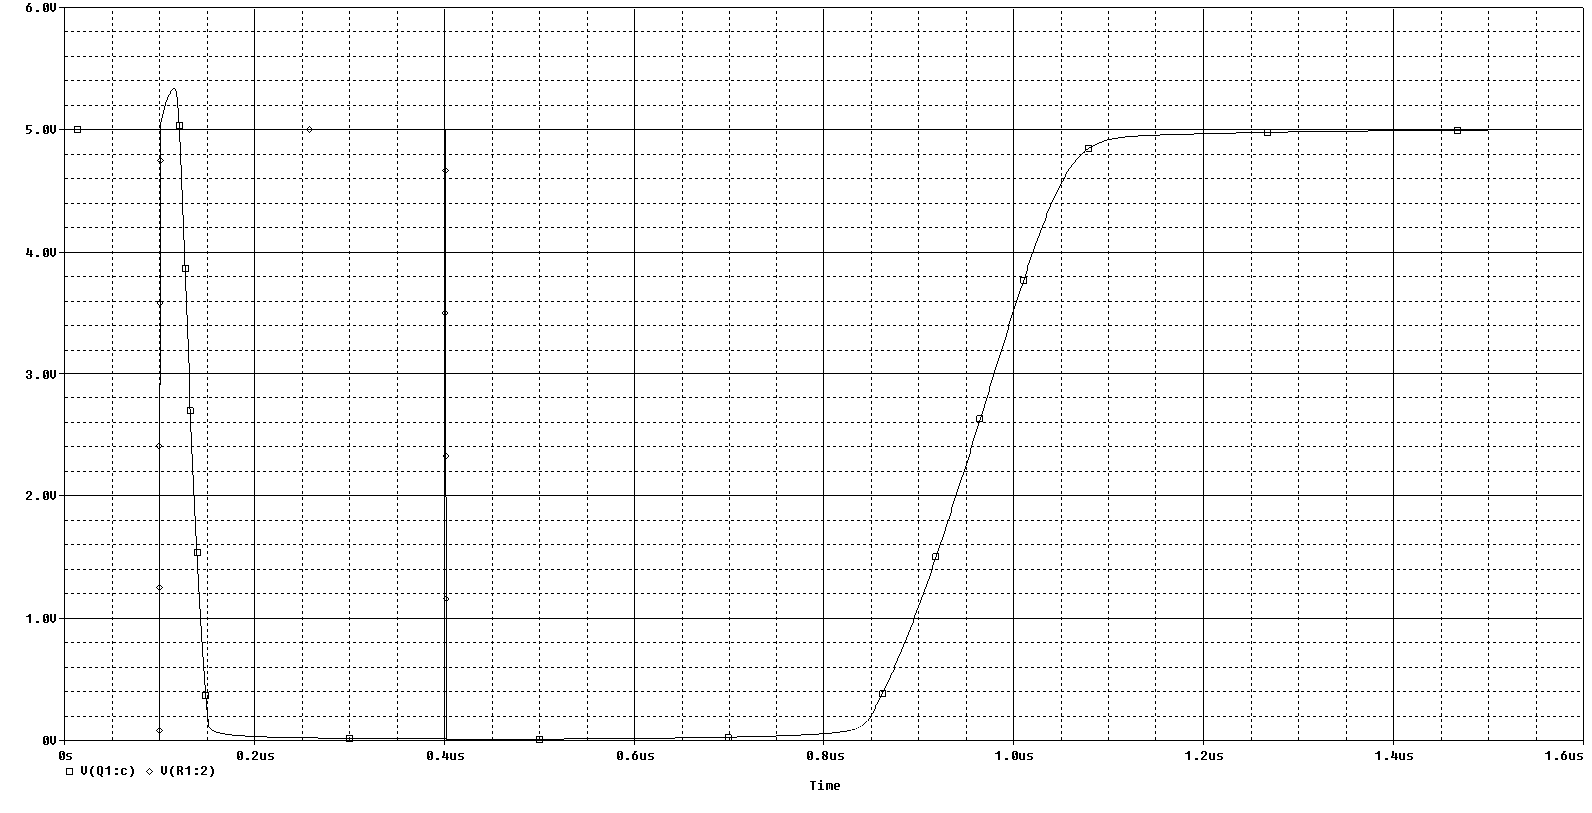
\includegraphics[width=\linewidth]{versuch5/spice/5411.png}
	\caption{Simulationsergebnis}
\end{figure}
Die Verzögerungszeit beim Einschalten des Transistors beträgt 70ns, die Verzögerung beim Ausschalten beträgt 1100ns. Der Transistor wird in Sättigung betrieben. Bis er umschalten kann, müssen erst überschüssige Ladungen aus ihm abfließen. Wenn man eine Diode einfügt, ergibt sich folgendes:
\subsubsection*{Simulation}
\begin{figure}[H]
	\centering
	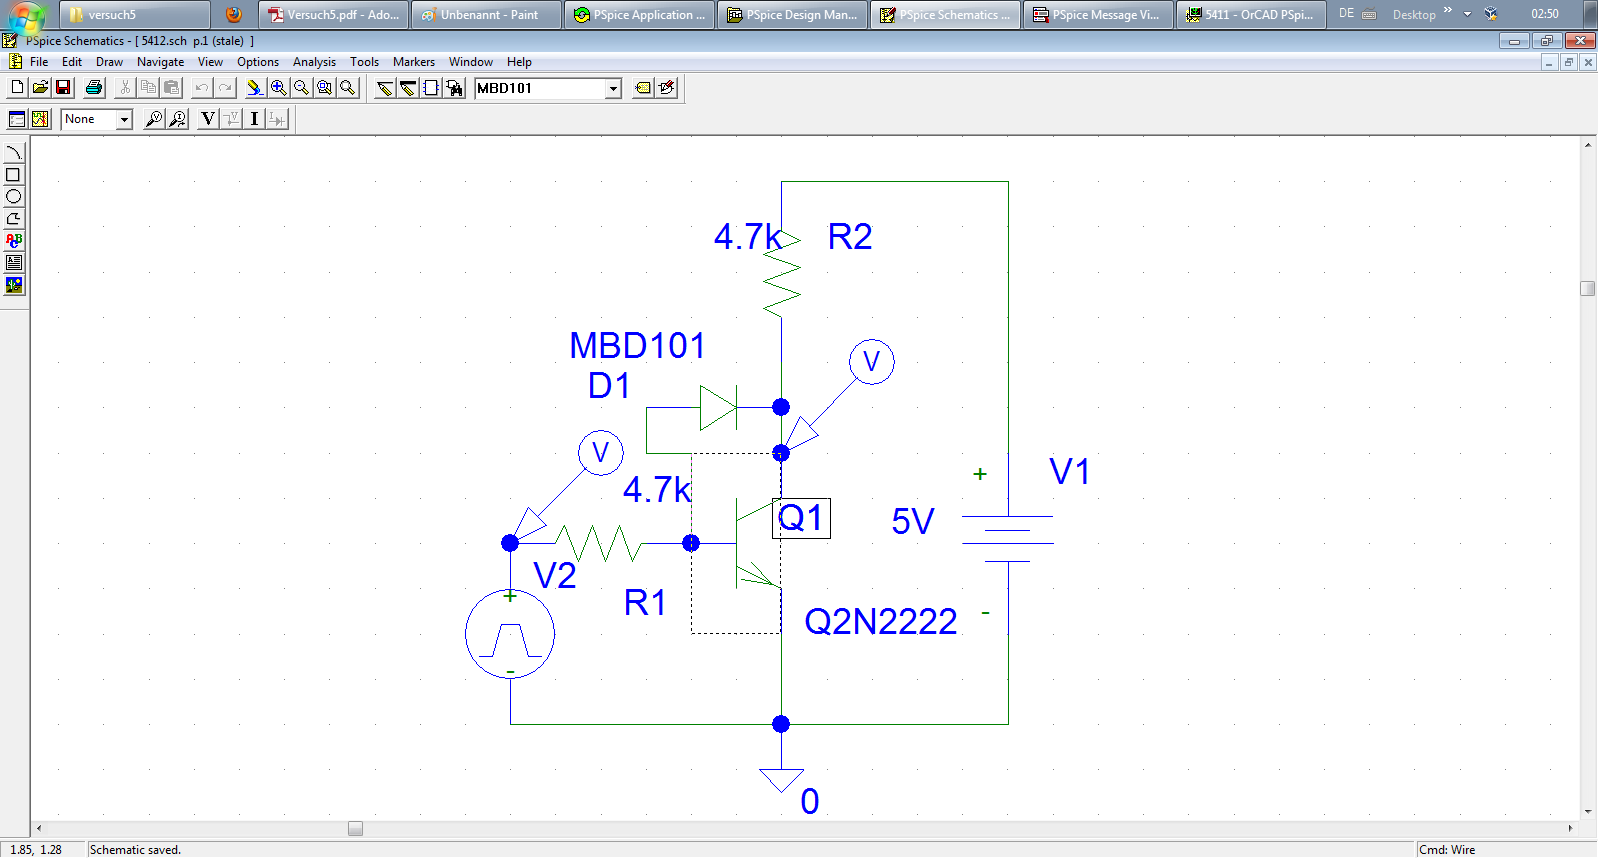
\includegraphics[width=\linewidth]{versuch5/spice/s5412.png}
	\caption{Schaltplan, wie im Skript vorgegeben}
\end{figure}
\begin{figure}[H]
	\centering
	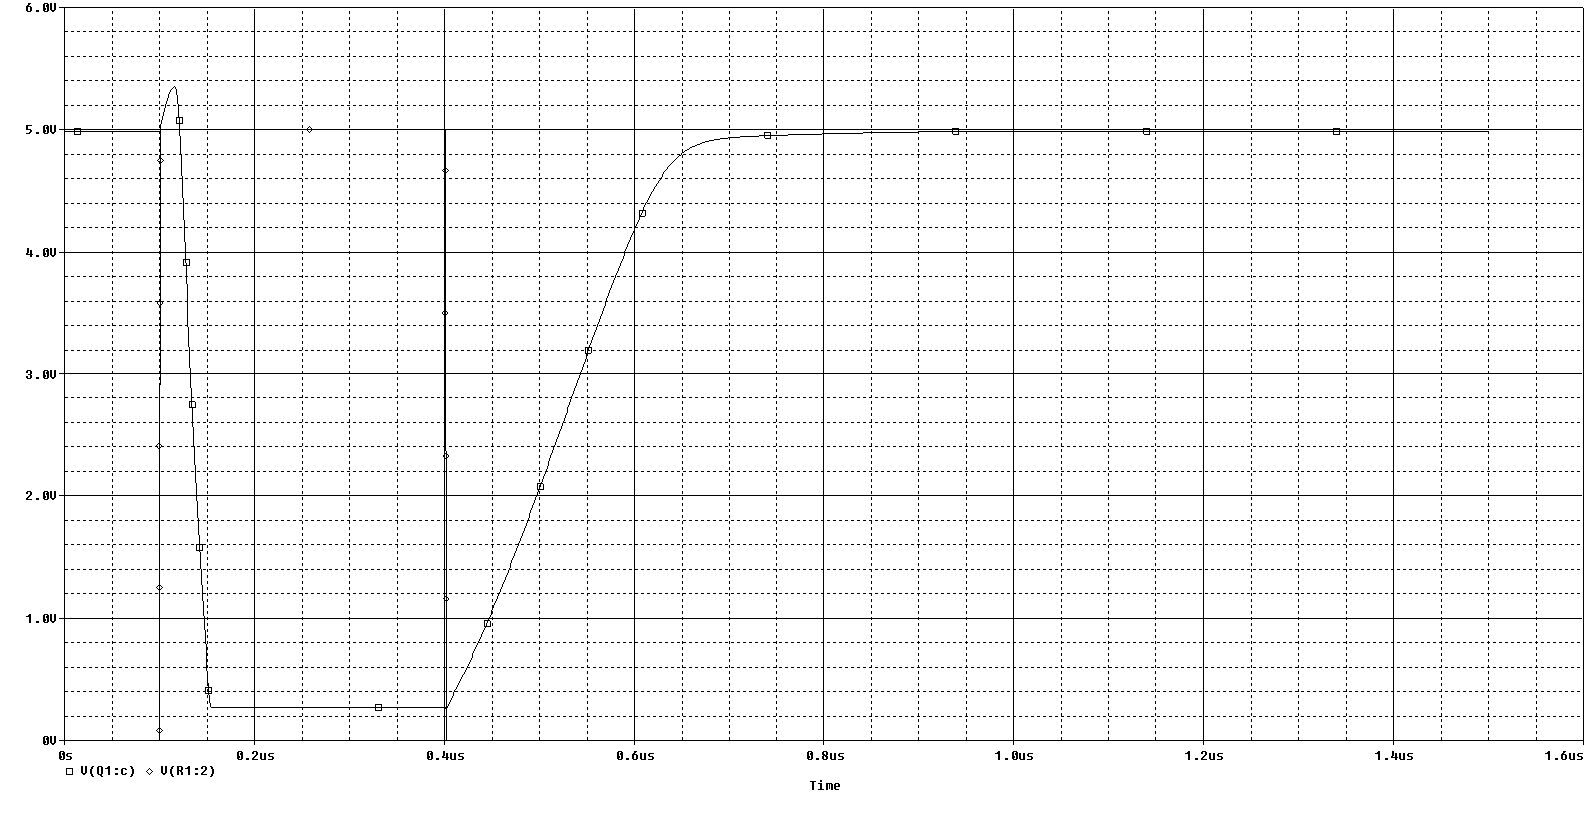
\includegraphics[width=\linewidth]{versuch5/spice/5412.png}
	\caption{Simulationsergebnis}
\end{figure}
Durch die Diode wird das Ausschalten deutlich beschleunigt, allerdings erreicht der Schalter jetzt nicht mehr die 0V, sondern nur noch 1.1V. Die Verwendung einer PN-Diode wäre hier fatal, da sie während ihrer Speicherzeit die Versorgungsspannung niederohmig mit dem Eingangssignal verbände.

\subsection{Transistor als Schalter mit induktiver Last}
\begin{figure}[H]
	\centering
	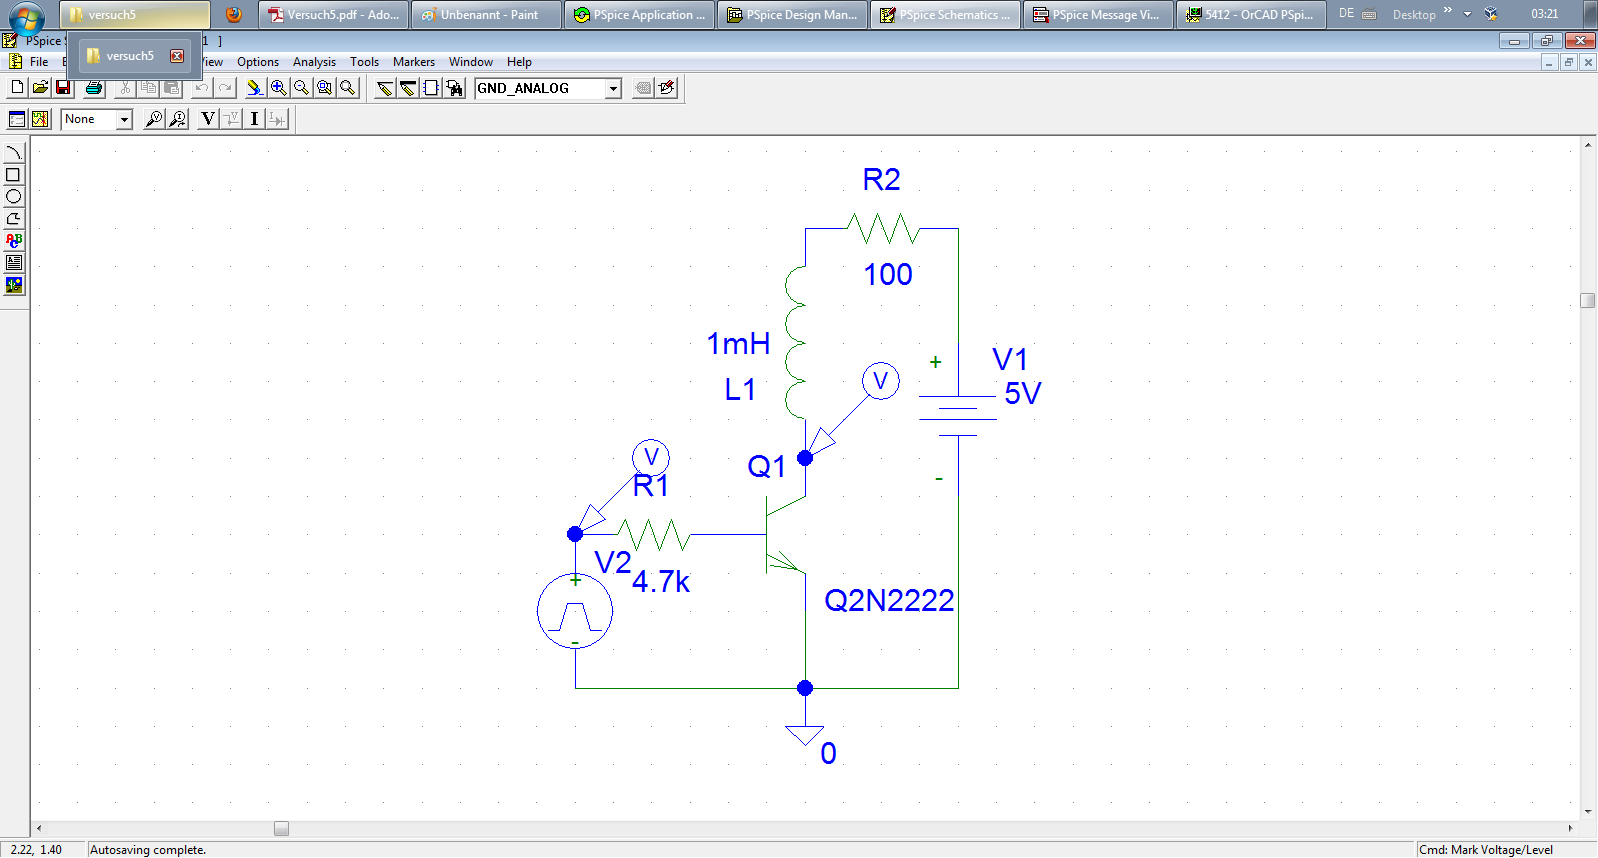
\includegraphics[width=\linewidth]{versuch5/spice/s5511.png}
	\caption{Schaltplan, wie im Skript vorgegeben}
\end{figure}
\begin{figure}[H]
	\centering
	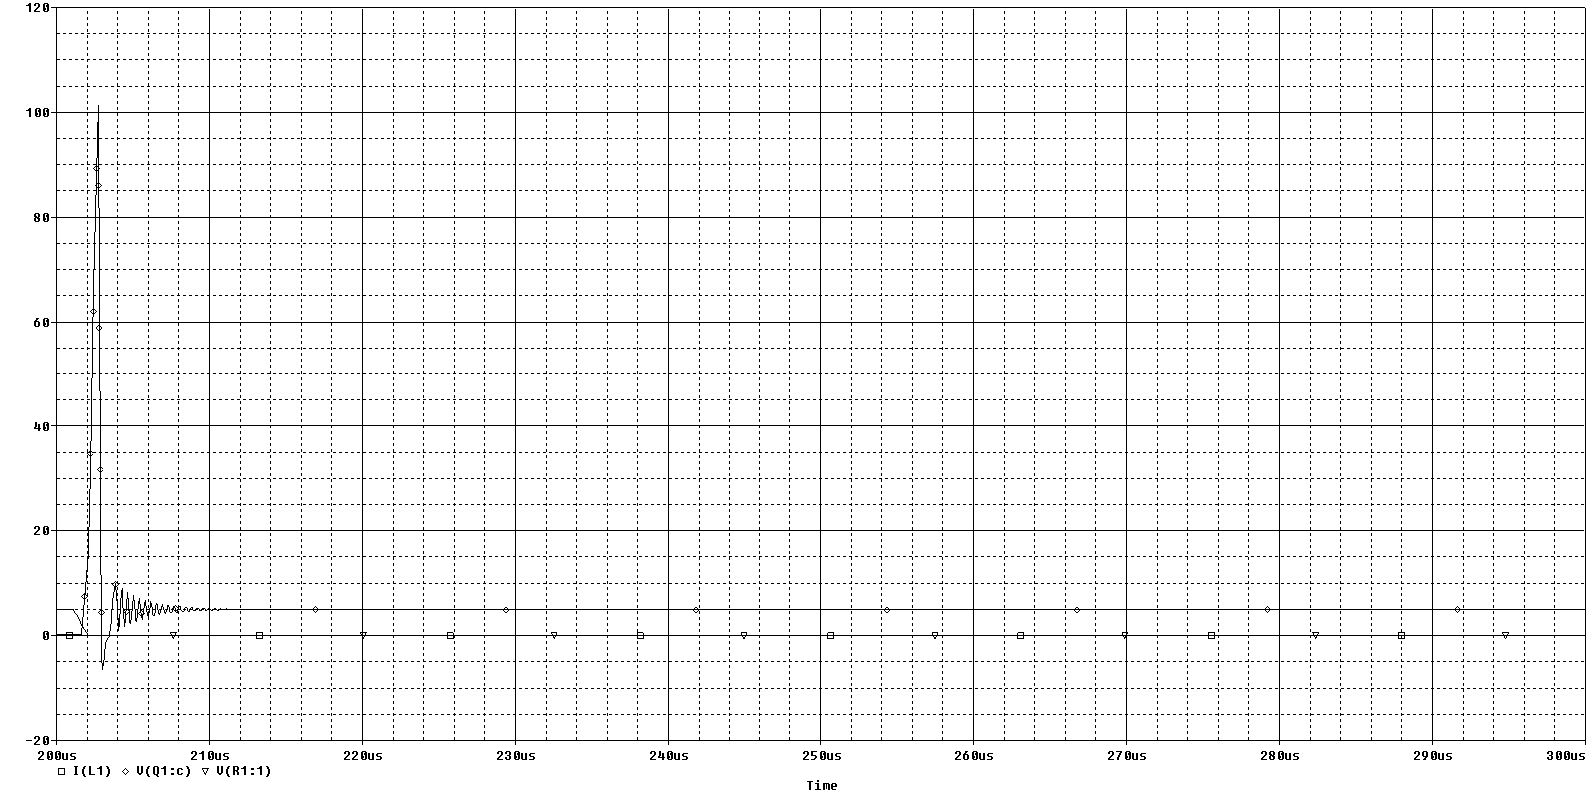
\includegraphics[width=\linewidth]{versuch5/spice/5511.png}
	\caption{Simulationsergebnis}
\end{figure}
\begin{figure}[H]
	\centering
	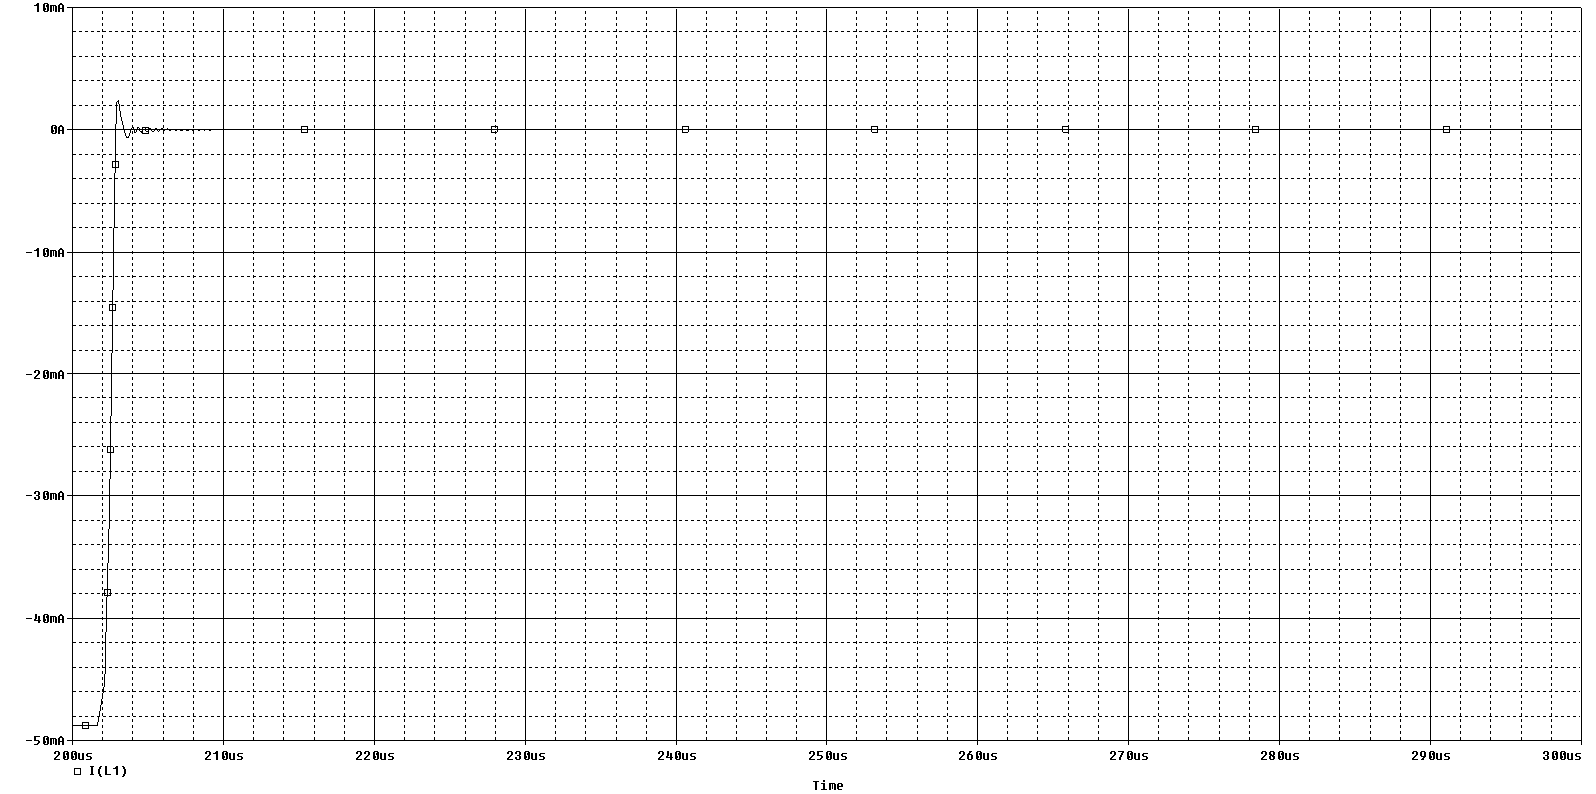
\includegraphics[width=\linewidth]{versuch5/spice/5511I.png}
	\caption{Simulationsergebnis: Strom}
\end{figure}
Der Transistor wird nicht lange überleben, weil er plötzlich gut 105V ableiten muss, wofür er sehr wahrscheinlich nicht gemacht war.\\ Die maximale Stromänderung wurde mit folgenden beiden Wertepaaren bestimmt (202.252\µs, -40.996mA) und (202.782\µs, -5.7515mA):
\[ \Delta I_{max}=\frac{-40.996+5.7515}{202.252-202.782}=-0.1819 \frac{A}{\µs}\]
Damit ergibt sich die Induzierte Spannung zu
\[ U_{IND} = -L*\frac{\Delta I}{\Delta t};\; L=1mH,\; \frac{\Delta I}{\Delta t}=-0.1819 \frac{A}{\µs} \]
\[ \Rightarrow \; U_{IND}=\frac{1mH*0.1819A}{1\µs}=\frac{0.1819HA}{1ms}=\frac{181.9HA}{1s}=181.9V \]
\begin{figure}[H]
	\centering
	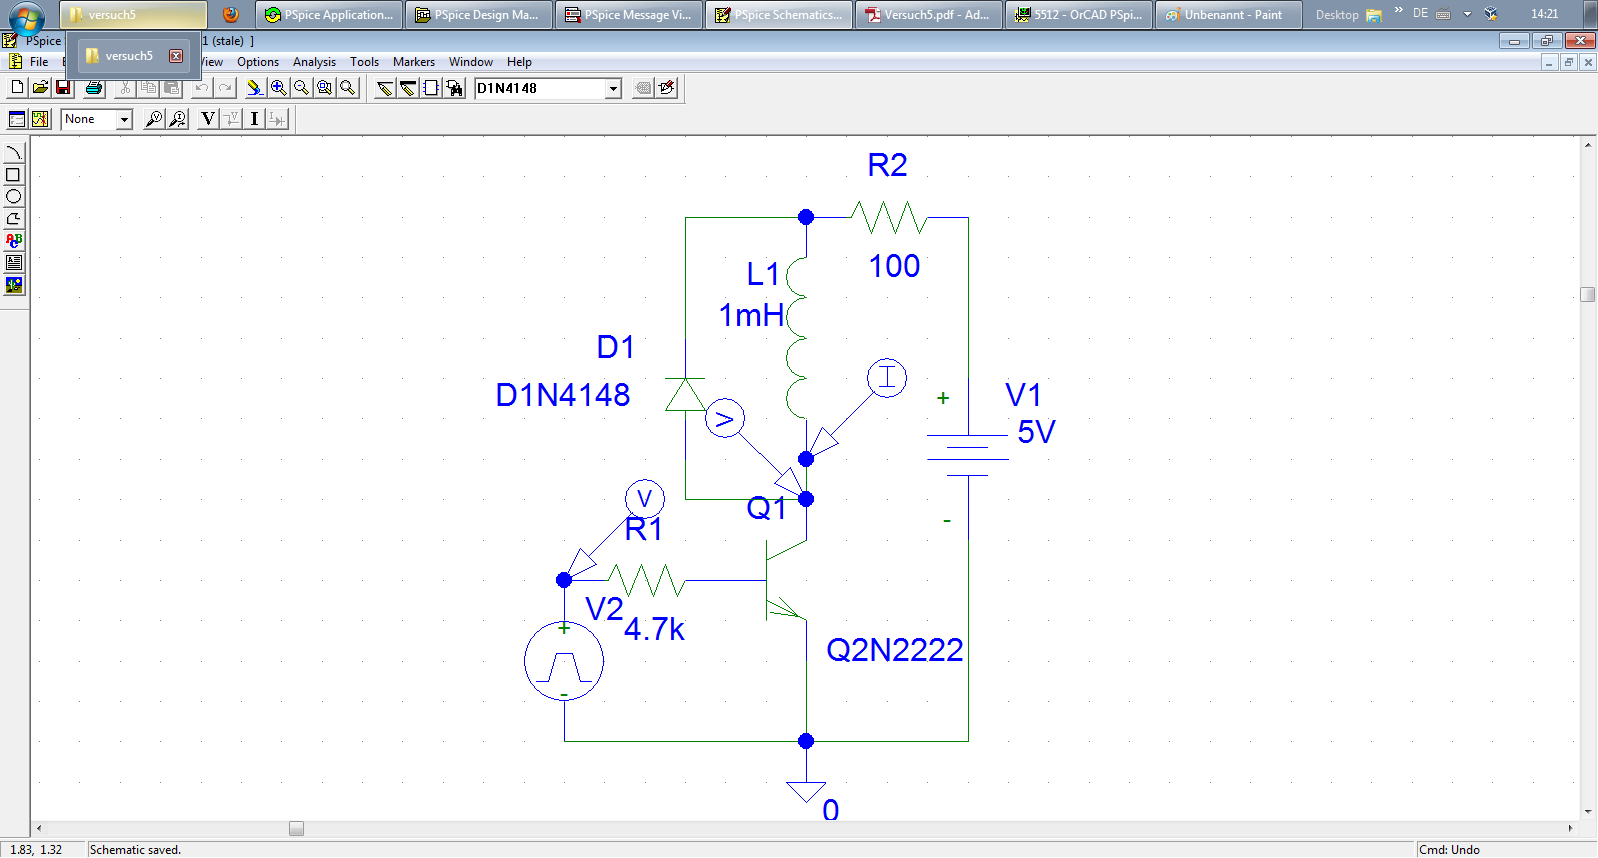
\includegraphics[width=\linewidth]{versuch5/spice/s5512.png}
	\caption{Schaltplan, mit Diode}
\end{figure}
\begin{figure}[H]
	\centering
	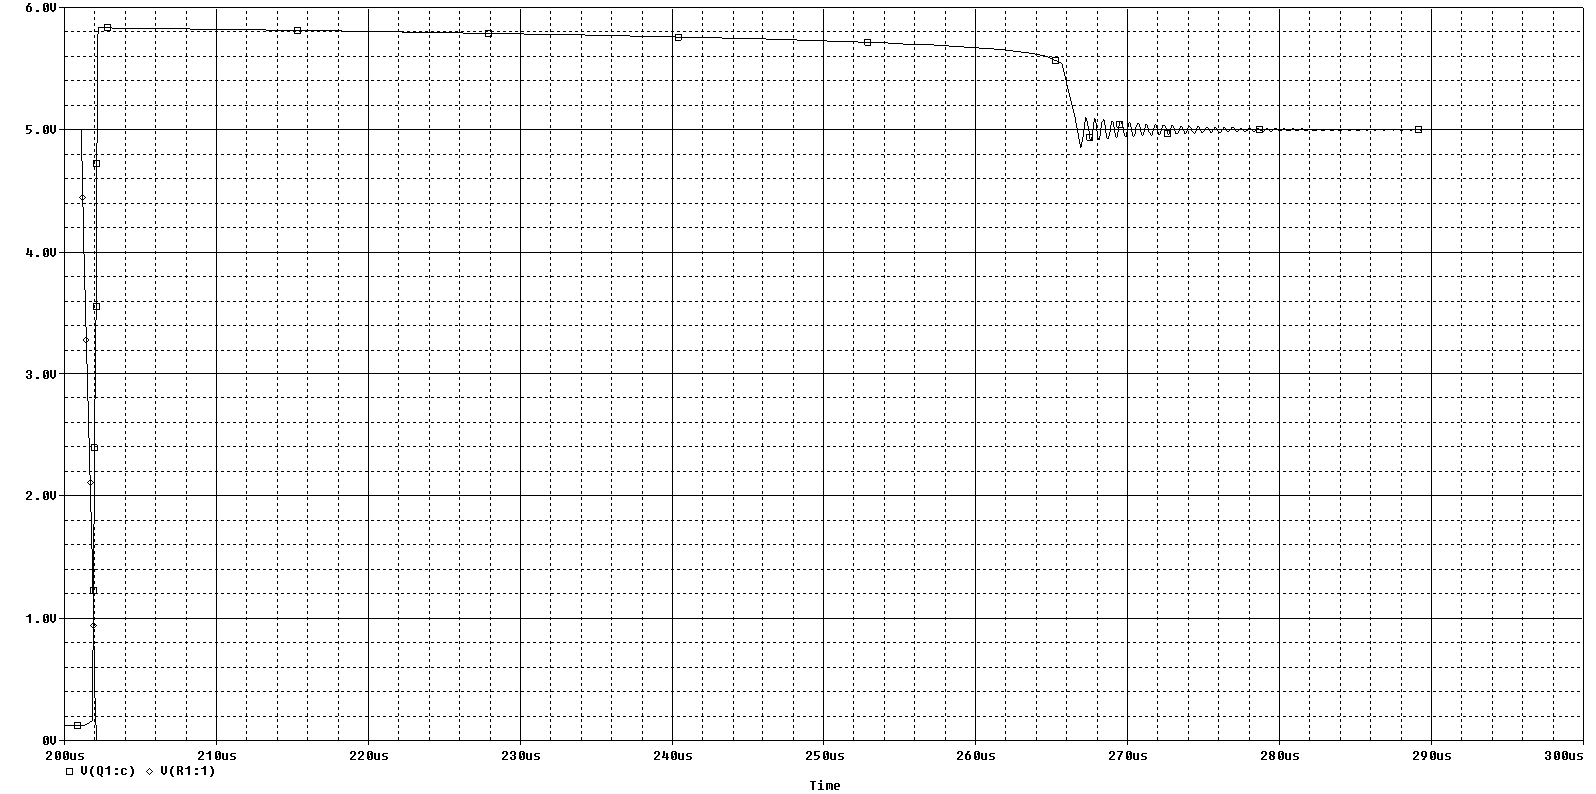
\includegraphics[width=\linewidth]{versuch5/spice/5512.png}
	\caption{Simulationsergebnis: Die Spannungsspitze wird durch die Diode abgeleitet}
\end{figure}
\begin{figure}[H]
	\centering
	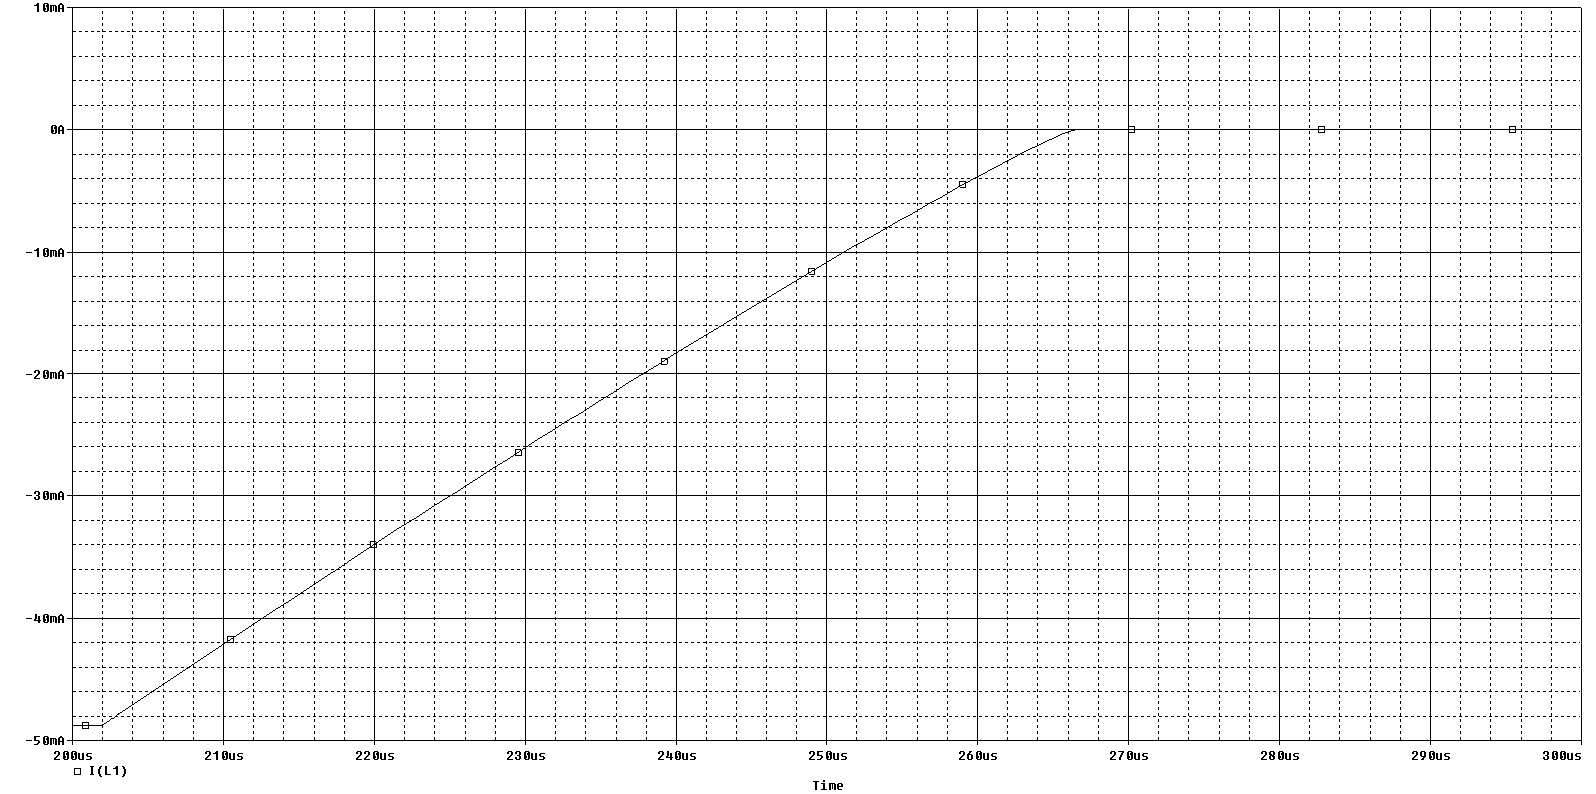
\includegraphics[width=\linewidth]{versuch5/spice/5512I.png}
	\caption{Simulationsergebnis: \Delta I deutlich geringer}
\end{figure}

































%}}}

